%% [Stats Project]

%% ================ load packages =============================================================
\documentclass[10pt, twoside, openleft]{article}
\usepackage[utf8]{inputenc}
\usepackage{titling}
\usepackage{titlesec}
\usepackage{fancyhdr}
\usepackage{amsmath, amsthm, amssymb, array}
\usepackage{thmtools}
\usepackage{calc}
\usepackage[width=16cm,height=20.5cm,left=2.5cm,right=2.5cm]{geometry}
\usepackage{tabu, colortbl}
\usepackage[table]{xcolor}
\usepackage{graphicx}
\usepackage[cache=false]{minted}
\usepackage{xpatch}
\usepackage{blindtext}
\usepackage{fancyhdr}
\usepackage{bold-extra}

\raggedbottom
\graphicspath{{./figures/}}
\setlength\textwidth{6.5in}

\xpatchcmd{\minted}{\VerbatimEnvironment}{\VerbatimEnvironment\let\itshape\relax}{}{}
\xpatchcmd{\minted}{\VerbatimEnvironment}{\VerbatimEnvironment\let\bfseries\relax}{}{}
\usemintedstyle{bw}

\pagestyle{fancy}
\renewcommand{\subsectionmark}[1]{\markboth{#1}{}}
\fancyhf{}
\fancyhead[LE,RO]{\raisebox{-0.5cm}{\filcenter\scshape\leftmark}}
\fancyhead[RE,LO]{\raisebox{-0.5cm}{\footnotesize\thepage}}
\renewcommand{\headrulewidth}{0pt}
\fancypagestyle{plain}{\fancyhead{}\renewcommand{\headrulewidth}{0pt}}
\titleformat{\section}[hang]{\filcenter\scshape\normalsize}{}{1pt}{}
\titleformat{\subsection}[hang]{\filcenter\scshape\LARGE}{}{1pt}{}

\newcommand{\alphahat}{\hat{\alpha}} %alphahat
\newcommand{\betahat}{\hat{\beta}} %betahat
\newcommand{\epsilonhat}{\hat{\epsilon}} %epsilonhat
\newcommand{\yhat}{\hat{y}} %yhat
\newcommand{\rhat}{\hat{r}} %rhat
\newcommand{\ybar}{\bar{y}} %ybar

%% ================ TITLE =====================================================================
%\setlength{\droptitle}{6cm}
\title{Testing for Linearity Between Major Category \& Income}
\author{Michael Šòdéké}
\date{\vspace{-14ex}}

\begin{document}
\maketitle

%% ================ ABSRACT ===================================================================
%% [0-main] block ...
%% -------------------------------------------------------------------------------------------\
\noindent\rule[-2.0\baselineskip]{\linewidth}{0.2pt}
\vspace{-3ex}
\begin{center}
\section{ABSTRACT}
\vspace{-3ex}
\end{center}
%% -------------------------------------------------------------------------------------------|

%% [1-summary] block ...
%% -------------------------------------------------------------------------------------------\
\noindent
\textbf{Method} \\
\textsc{case i} involved the use of the ANCOVA (one-way) model that helped
generate values for the response variable. Parameter estimates,
$\alphahat$ and $\betahat$, and the degrees of freedom, $df$, were calculated.
The MSE was found after calculating the sum of squares. A hypothesis test was
conducted to determine if there truly existed a linear relation between
\textbf{major category} and \textbf{income}. Influence diagnostics were used to
identify any data points that effected the outcome of the model. Finally, model
validation was explored to determine which parameters were relevant to the model.
The model was then adjusted to accommodate for the removal of one of the features. 
\smallskip

\noindent
\textbf{Conclusion} \\
\textsc{case i} revealed a weak linear relation between the regressors and
the response variable. However, \textsc{case i} resutls only
state that no \emph{linear} relation exists, but does not state that
no \emph{other} relation exists. More adavnced mathematical modeling techniques
are needed to discover what this true relation would be. Adjusted results in
\textsc{case ii} reached a similar conclusion: there is no sign of linearity in
the model.
\smallskip

\noindent\rule[0.5ex]{\linewidth}{0.2pt}
\bigskip
\bigskip
%% -------------------------------------------------------------------------------------------|

%% ================ CASE 1 ====================================================================
%% [0-main] block ...
%% -------------------------------------------------------------------------------------------\
\begin{center}
\section{CASE I: PRE-MODEL VALIDATION}
\vspace{-5ex}
\end{center}
%% -------------------------------------------------------------------------------------------|

%% [A-title] block ...
%% -------------------------------------------------------------------------------------------\
\begin{center}
\subsection{introduction}
\vspace{-3ex}
\end{center}
%% -------------------------------------------------------------------------------------------|

%% [B-paragraph] block ...
%% -------------------------------------------------------------------------------------------\
\noindent
\textsc{case i} involves the use of the ANCOVA (one-way) model that will help
gnerate values for the response variable. From this model, the parameter estimates,
$\alphahat$ and $\betahat$, and the degrees of freedom, $df$, can be calculated.
Next, the MSE is found after calculating the sum of squares. A hypothesis test is
conducted to determine if there truely exists a linear relation between
\textbf{major category} and \textbf{income}. Influence diagnostics will be used to
identify any data points that are effecting the outcome of the model. Finally, model
validation is explored to determine which parameters are relevant to the model.
\smallskip
%% -------------------------------------------------------------------------------------------|

%% [A-title] block ...
%% -------------------------------------------------------------------------------------------\
\begin{center}
\subsection{ancova one-way (unbalanced) model}
\vspace{-3ex}
\end{center}
%% -------------------------------------------------------------------------------------------|

%% [B-paragraph] block ...
%% -------------------------------------------------------------------------------------------\
\noindent
Since \textbf{major category} is categorical and both \textbf{perc college jobs} and
\textbf{perc non college jobs} are numeric, the best option is to use the ANCOVA
(one-way) model with $q = 2$ covariates. The model can be expressed in mathematical
notation as
\smallskip

\begin{equation*}
\begin{aligned}
y_{ij} = \mu + \alpha_{i} + \beta x_{ij1} + \beta x_{ij2} + \epsilon_{ij}
\end{aligned}
\end{equation*}
\smallskip

where:
\begin{equation*}
\begin{aligned}
& i = 1,2,...,k \ \text{observations}, \\
& j = 1,2,...,n \ \text{features}
\end{aligned}
\end{equation*}
\smallskip

\noindent
Here is the model expressed in matrix notation
\begin{equation*}
\begin{aligned}
\mathbf{y} = \mathbf{Z} \mathbf{\alpha} + \mathbf{X} \mathbf{\beta} + \mathbf{\epsilon}
\end{aligned}
\end{equation*}
\smallskip

where:
\begin{equation*}
\begin{aligned}
& \mathbf{Z} =
\left[ \begin{array}{ccccc}
    1 & 0 & 0 & \cdots & 0 \\
    \vdots & \vdots & \vdots &  & \vdots \\
    1 & 1 & 0 & \cdots & 0 \\
    1 & 1 & 0 & \cdots & 0 \\
    \vdots & \vdots & \vdots &  & \vdots \\
    1 & 0 & 0 & \cdots & 1, 
\end{array}\right]
, & \mathbf{\alpha} =
\left[ \begin{array}{c}
    \mu \\
    \alpha_{1}
\end{array}\right] \\
& & \\
& \mathbf{X} =
\left[ \begin{array}{ccccc}
    x_{111} & x_{112} \\
    x_{121} & x_{122} \\
    \vdots & \vdots \\
    x_{kn1} & x_{kn2}
\end{array}\right]
, & \mathbf{\beta} =
\left[ \begin{array}{c}
    \betahat_{1} \\
    \betahat_{2} 
\end{array}\right]
\end{aligned}
\end{equation*}
\smallskip

Take note that $\mathbf{Z}$ is assumed to be rank-deficient and $\mathbf{X}$ is full-rank.
Therefore $\mathbf{Z}$ will be reparameterized to become full-rank. Below is the ANCOVA
model in code.
%% -------------------------------------------------------------------------------------------|

%% [C-code] block ...
%% -------------------------------------------------------------------------------------------\
\definecolor{lightgrey}{rgb}{0.972,0.972,0.972}
\begin{minted}[linenos=false, bgcolor=lightgrey, fontfamily=qcr, fontsize=\footnotesize]{r}
df <- college
df <- college %>% dplyr::select(median, major_category, perc_college_jobs, perc_non_college_jobs)
df <- na.omit(df)
df <- arrange(df, major_category)
df[,2] <- as.factor(df[,2])
lapply(df, head)
df %>% group_by(major_category, .add=TRUE) %>% group_nest()

Z <- as.matrix( ( model.matrix( median ~ major_category, data=df) ) ) # full-rank
X <- as.matrix( cbind(df$perc_college_jobs, df$perc_non_college_jobs) ) # full-rank
colnames(X) <- c("perc_college_jobs", "perc_non_college_jobs")
Y <- df$median
\end{minted}
%% -------------------------------------------------------------------------------------------|

%% [A-title] block ...
%% -------------------------------------------------------------------------------------------\
\begin{center}
\subsection{estimating parameters $\alpha$ \& $\beta$}
\vspace{-3ex}
\end{center}
%% -------------------------------------------------------------------------------------------|

%% [B-paragraph] block ...
%% -------------------------------------------------------------------------------------------\
\noindent
In order to generate values for the response variable, $\yhat$, $\alpha$ and $\beta$ need to be
estimated. In other words, to find $\alpha$ and $\beta$, the estimates $\alphahat$ and $\betahat$
must be calculated.
\smallskip

Now that $\mathbf{Z}$ is full-rank, there is no need to use the general inverse of $\mathbf{Z}$,
$(\mathbf{Z}^{'} \mathbf{Z})^{-}$. Therefore, $\alphahat$ can be calculated as follows
\begin{equation*}
\begin{aligned}
\alphahat = ( \mathbf{Z}^{'} \mathbf{Z} )^{-} ( \mathbf{Z}^{'} \mathbf{y} ) -
( \mathbf{Z}^{'} \mathbf{Z} )^{-} ( \mathbf{Z}^{'} \mathbf{X} \betahat )
\end{aligned}
\end{equation*}
\smallskip

\noindent
The equation for $\alphahat$ can be used for estimating $\betahat$
\begin{equation*}
\begin{aligned}
\betahat & = ( \mathbf{X}^{'} \mathbf{Z} ) [ ( \mathbf{Z}^{'} \mathbf{Z})^{-}
( \mathbf{Z}^{'} \mathbf{y} ) - ( \mathbf{Z}^{'} \mathbf{Z} ) ( \mathbf{Z}^{'} \mathbf{X}
\betahat ) ] + \mathbf{X}^{'} \mathbf{X} \betahat = \mathbf{X}^{'} \mathbf{y} \\
	 & = ( \mathbf{X}^{'} \mathbf{Z} ) [ (\mathbf{Z}^{'} \mathbf{Z} )^{-}
( \mathbf{Z}^{'} \mathbf{y} ) ] - ( \mathbf{X}^{'} \mathbf{Z} )
[ ( \mathbf{Z}^{'} \mathbf{Z} )^{-} ( \mathbf{Z}^{'} \mathbf{X}
\betahat ) ] + \mathbf{X}^{'} \mathbf{X} \betahat = \mathbf{X}^{'} \mathbf{y} \\
	 & = \mathbf{X}^{'} [ \mathbf{Z} ( \mathbf{Z}^{'} \mathbf{Z} )^{-}
( \mathbf{Z}^{'} \mathbf{y} ) ] + \mathbf{X}^{'} [ \mathbf{I} - \mathbf{Z}
( \mathbf{Z}^{'} \mathbf{Z} )^{'} \mathbf{Z}^{'} ] \mathbf{X} \betahat = \mathbf{X}^{'} \mathbf{y} \\
	 & = \mathbf{X}^{'} ( \mathbf{P} ) \mathbf{y} + \mathbf{X}^{'} [ \mathbf{I} - \mathbf{P}]
\mathbf{X} \betahat = \mathbf{X}^{'} \mathbf{y} \\
	 & = \mathbf{X}^{'} [ \mathbf{I} - \mathbf{P} ] \mathbf{X} \betahat = \mathbf{X}^{'} \mathbf{y}
- \mathbf{X}^{'} ( \mathbf{P} ) \mathbf{y} \\
	 & = \mathbf{X}^{'} [ \mathbf{I} - \mathbf{P} ] \mathbf{X} \betahat = \mathbf{X}^{'}
[ \mathbf{I} - \mathbf{P} ] \mathbf{y} \\
	 & = \mathbf{E}_{xx}^{-} \mathbf{e}_{xy}
\end{aligned}
\end{equation*}
\smallskip

\noindent
For convenience, the ANCOVA model is reconstructed as
\begin{equation*}
\begin{aligned}
\mathbf{y} = \mathbf{U} \mathbf{\Gamma} + \mathbf{\epsilon}
\end{aligned}
\end{equation*}
\smallskip

where:
\begin{equation*}
\begin{aligned}
& \mathbf{U} =
\left[ \begin{array}{c}
    \mathbf{Z}, \ \mathbf{X}
\end{array}\right],
& \mathbf{\Gamma} =
\left[ \begin{array}{c}
    \alphahat \\
    \betahat
\end{array}\right]
\end{aligned}
\end{equation*}
\smallskip
%% -------------------------------------------------------------------------------------------|

%% [C-code] block ...
%% -------------------------------------------------------------------------------------------\
\definecolor{lightgrey}{rgb}{0.972,0.972,0.972}
\begin{minted}[linenos=false, bgcolor=lightgrey, fontfamily=qcr, fontsize=\footnotesize]{r}
P <- Z %*% ginv(t(Z) %*% Z) %*% t(Z)
I <- diag(dim(P)[1])
B_ <- solve(t(X) %*% (I - P) %*% X) %*% (t(X) %*% (I - P) %*% Y); colnames(B_) <- "Estimates"
A_ <- ginv(t(Z) %*% Z) %*% (t(Z) %*% Y) - ginv(t(Z) %*% Z) %*% (t(Z) %*% (X %*% B_))
rownames(A_) <- colnames(Z)
rownames(B_) <- colnames(X)
U <- cbind(Z, X)
GAMMA <- rbind(A_, B_)
Y_ <- U %*% GAMMA
\end{minted}
%% -------------------------------------------------------------------------------------------|

%% [A-title] block ...
%% -------------------------------------------------------------------------------------------\
\begin{center}
\subsection{degrees of freedom}
\vspace{-3ex}
\end{center}
%% -------------------------------------------------------------------------------------------|

%% [B-paragraph] block ...
%% -------------------------------------------------------------------------------------------\
\noindent
The degrees of freedom for the error is $df = n-k$. This can be used for generating
values for the MSE, $\sigma^{2}$.
\bigskip
%% -------------------------------------------------------------------------------------------|

%% [C-code] block ...
%% -------------------------------------------------------------------------------------------\
\definecolor{lightgrey}{rgb}{0.972,0.972,0.972}
\begin{minted}[linenos=false, bgcolor=lightgrey, fontfamily=qcr, fontsize=\footnotesize]{r}
n <- nrow(U); k <- qr(U)$rank
\end{minted}
%% -------------------------------------------------------------------------------------------|

%% [A-title] block ...
%% -------------------------------------------------------------------------------------------\
\begin{center}
\subsection{sum of squares}
\vspace{-3ex}
\end{center}
%% -------------------------------------------------------------------------------------------|

%% [B-paragraph] block ...
%% -------------------------------------------------------------------------------------------\
\noindent
Next, the sum of squares are calculated
\begin{equation*}
\begin{aligned}
SSE & = SS_{res} = \left( \mathbf{y} - \mathbf{\yhat} \right)^{'} \left( \mathbf{y} -
\mathbf{\yhat} \right) \\
SSR & = SS_{reg} = \left( \mathbf{y} - \mathbf{\ybar} \right)^{'} \left( \mathbf{y} -
\mathbf{\ybar} \right) \\
SST & = SS_{tot} = SS_{res} + SS_{reg} \\
R^{2} & = \frac{ SS_{res} }{ SS_{reg} } 
\end{aligned}
\end{equation*}
\smallskip
%% -------------------------------------------------------------------------------------------|

%% [C-code] block ...
%% -------------------------------------------------------------------------------------------\
\definecolor{lightgrey}{rgb}{0.972,0.972,0.972}
\begin{minted}[linenos=false, bgcolor=lightgrey, fontfamily=qcr, fontsize=\footnotesize]{r}
ss.res <- (t(Y) %*% Y) - (t(GAMMA) %*% t(U) %*% Y)
ss.reg <- t(Y_ - mean(Y)) %*% (Y_ - mean(Y))
ss.tot <- ss.res + ss.reg
R.2 <- ss.res/ss.reg
\end{minted}
%% -------------------------------------------------------------------------------------------|

%% [A-title] block ...
%% -------------------------------------------------------------------------------------------\
\begin{center}
\subsection{mean squares}
\vspace{-3ex}
\end{center}
%% -------------------------------------------------------------------------------------------|

%% [B-paragraph] block ...
%% -------------------------------------------------------------------------------------------\
\noindent
Using the formula for the $SS_{res}$, calculate the MSE
\begin{equation*}
\begin{aligned}
MSE & = \sigma^{2} \\
    & = \frac{ SS_{res} }{ k \left( n-1 \right) }
\end{aligned}
\end{equation*}
\smallskip

\noindent
Now use the MSE to calculate the standard errors for the estimates in $\Gamma$
\begin{equation*}
\begin{aligned}
SE_{\Gamma} = \sqrt{ diag(\sigma^{2} ( \mathbf{U}^{'} \mathbf{U})^{-} ) }
\end{aligned}
\end{equation*}
\smallskip
%% -------------------------------------------------------------------------------------------|

%% [C-code] block ...
%% -------------------------------------------------------------------------------------------\
\definecolor{lightgrey}{rgb}{0.972,0.972,0.972}
\begin{minted}[linenos=false, bgcolor=lightgrey, fontfamily=qcr, fontsize=\footnotesize]{r}
ms.res <- ss.res/(n-k)
SE.. <- matrix( sqrt( diag( ms.res[1] * solve(t(U) %*% U) ) ) );  colnames(SE..) <- "Std. Error"
\end{minted}
%% -------------------------------------------------------------------------------------------|

%% [A-title] block ...
%% -------------------------------------------------------------------------------------------\
\begin{center}
\subsection{hypothesis test}
\vspace{-3ex}
\end{center}
%% -------------------------------------------------------------------------------------------|

%% [B-paragraph] block ...
%% -------------------------------------------------------------------------------------------\
\noindent
To determine if there exists a linear relation between the regressors and the
response variable, a hypothesis test is needed, namely a t-test.
\smallskip

\noindent
The hypothesis test is constructed as follows
\begin{equation*}
\begin{aligned}
& H_{0}: \Gamma = 0 \ \text{no linear relation.} \\
& H_{a}: \Gamma \neq 0 \ \text{linear relation exists.}
\end{aligned}
\end{equation*}
\smallskip

where:
\begin{equation*}
\begin{aligned}
\Gamma = 
\left[ \begin{array}{c}
    \alpha \\
    \beta_{1} \\
    \beta_{2} 
\end{array}\right]
\end{aligned}
\end{equation*}
\smallskip

\noindent
Next, construct the t-test
\begin{equation*}
\begin{aligned}
t_{test} = \frac{ \Gamma - 0 }{ SE_{\Gamma} }
\end{aligned}
\end{equation*}
\smallskip

\noindent
Reject the null hypothesis, $H_{0}$, if $t_{test} \geq t_{1-\alpha, n-k}$.
%% -------------------------------------------------------------------------------------------|

%% [C-code] block ...
%% -------------------------------------------------------------------------------------------\
\definecolor{lightgrey}{rgb}{0.972,0.972,0.972}
\begin{minted}[linenos=false, bgcolor=lightgrey, fontfamily=qcr, fontsize=\footnotesize]{r}
t.B_ <- GAMMA / SE..;  colnames(t.B_) <- "t value"
t.alpha <- qt(1-(0.05/2), df=n-k)
p_val.B_ <- 2*pt(-abs(t.B_), df=n-k);  colnames(p_val.B_) <- "Pr(>|t|)"
p_val.alpha <- 2*pt(-abs(t.alpha), df=n-k)
\end{minted}
%% -------------------------------------------------------------------------------------------|

%% [D0-result-ctext] block ...
%% -------------------------------------------------------------------------------------------\
\definecolor{lightgrey}{rgb}{0.952,0.952,0.952}
\begin{minted}[linenos=false, bgcolor=lightgrey, fontfamily=qcr, fontsize=\footnotesize]{r}
cbind(t.B_, p_val.B_)

                                                      t value     Pr(>|t|)
(Intercept)                                        5.49281690 1.600036e-07
major_categoryArts                                -1.17028901 2.436925e-01
major_categoryBiology & Life Science              -0.05664043 9.549050e-01
major_categoryBusiness                             0.96319248 3.369609e-01
major_categoryCommunications & Journalism         -0.31068316 7.564616e-01
major_categoryComputers & Mathematics             -1.90276400 5.893763e-02
major_categoryEducation                           -1.20920870 2.284358e-01
major_categoryEngineering                         -0.83124453 4.071225e-01
major_categoryHealth                              -0.77897389 4.371904e-01
major_categoryHumanities & Liberal Arts           -2.06184950 4.090272e-02
major_categoryIndustrial Arts & Consumer Services -0.57984119 5.628691e-01
major_categoryInterdisciplinary                   -1.54316186 1.248439e-01
major_categoryLaw & Public Policy                 -1.13011064 2.601867e-01
major_categoryPhysical Sciences                   -0.70983383 4.788806e-01
major_categoryPsychology & Social Work            -1.04710528 2.966917e-01
major_categorySocial Science                      -0.82522474 4.105205e-01
perc_college_jobs                                 -1.12842757 2.608943e-01
perc_non_college_jobs                             -0.22803152 8.199242e-01
\end{minted}
%% -------------------------------------------------------------------------------------------|

%% [A-title] block ...
%% -------------------------------------------------------------------------------------------\
\begin{center}
\subsection{influencial observations and leverage}
\vspace{-3ex}
\end{center}
%% -------------------------------------------------------------------------------------------|

%% [B-paragraph] block ...
%% -------------------------------------------------------------------------------------------\
\noindent
To prevent model misspecification, employ influence diagnostic measures
to identify outliers effecting the one-way ANCOVA model. These measures include
leverages, $h_{ii}$, residuals, $\epsilonhat_{i}$, studentized residuals,
$\hat{r}_{i}$, and Cook's Distance, $D_{i}$.
\smallskip

These diagnstic tools are calculated below
\begin{equation*}
\begin{aligned}
\mathbf{H} = \mathbf{X} ( \mathbf{X}^{'} \mathbf{X} ) \mathbf{X}^{'}
\end{aligned}
\end{equation*}

\begin{equation*}
\begin{aligned}
h_{ii} = diag(\mathbf{H}), \ h_{ii} \geq \frac{ 2 ( k+1 ) }{ n }
\end{aligned}
\end{equation*}

\begin{equation*}
\begin{aligned}
\epsilonhat_{i} = \mathbf{y} - \mathbf{\yhat}
\end{aligned}
\end{equation*}

\begin{equation*}
\begin{aligned}
\rhat_{i} = \frac{ \epsilonhat_{i} }{ \sqrt{ \sigma^{2} ( 1 - h_{ii} ) } }
\end{aligned}
\end{equation*}

\begin{equation*}
\begin{aligned}
D_{i} = \left( \frac{ \rhat^{2} }{ k+1 } \right) \left( \frac{ h_{ii} }{ 1 - h_{ii} } \right)
\end{aligned}
\end{equation*}
\smallskip
%% -------------------------------------------------------------------------------------------|

%% [C-code] block ...
%% -------------------------------------------------------------------------------------------\
\definecolor{lightgrey}{rgb}{0.972,0.972,0.972}
\begin{minted}[linenos=false, bgcolor=lightgrey, fontfamily=qcr, fontsize=\footnotesize]{r}
H <- X %*% solve(t(X) %*% X) %*% t(X)

create.hii <- function(mat=NULL)
{
	vec <- matrix(rep(0, nrow(mat)))
	for (i in 1:nrow(mat))
		for (j in 1:ncol(mat))
			if ( i == j)
				vec[i] <- mat[i,j] 
	vec
}

hii <- create.hii(mat=H) # leverage
e_ <- Y - Y_; # residual
r_ <- e_/sqrt(ms.res[1] * (1 - hii)) # studentized residual
D_ <- ((r_^2)/(k+1)) * ((hii)/(1-hii)) # Cook's distance
inf.measures <- cbind(head(Y), head(Y_), head(e_), head(hii), head(r_),  head(D_))
colnames(inf.measures) <- c("yi", "yi_", "ei_", "hii", "ri_", "Di_")
infl <- c( "hii_LEVERAGE"=(2*(k + 1))/n )
\end{minted}
%% -------------------------------------------------------------------------------------------|

%% [D0-result-ctext] block ...
%% -------------------------------------------------------------------------------------------\
\definecolor{lightgrey}{rgb}{0.952,0.952,0.952}
\begin{minted}[linenos=false, bgcolor=lightgrey, fontfamily=qcr, fontsize=\footnotesize]{r}
list(infl, inf.measures)

[[1]]
hii_LEVERAGE
   0.2209302

[[2]]
     yi      yi_        ei_         hii         ri_          Di_
1 33000 42216.23  -9216.231 0.012015861 -0.81692462 4.271843e-04
2 58000 45641.31  12358.687 0.008332640  1.09343497 5.287482e-04
3 40000 43851.68  -3851.682 0.006055751 -0.34038706 3.715339e-05
4 65000 45094.40  19905.600 0.009234717  1.76194968 1.522952e-03
5 45000 43943.40   1056.604 0.005921398  0.09336961 2.733135e-06
6 31000 41124.02 -10124.018 0.026722668 -0.90414531 1.181316e-03
\end{minted}
%% -------------------------------------------------------------------------------------------|

%% [B-paragraph] block ...
%% -------------------------------------------------------------------------------------------\
\noindent
In \textsc{figure 1} the \emph{residuals vs. fitted} graph shows a faint pattern that
appears to be either \emph{stochastic} or \emph{sinusoidal}. In addition, hardly
any outliers exist in the \emph{standardized residuals vs. leverage} graph.
\bigskip
%% -------------------------------------------------------------------------------------------|

%% [D2-result-image] block ...
%% -------------------------------------------------------------------------------------------\
\begin{figure}[H]
\centering
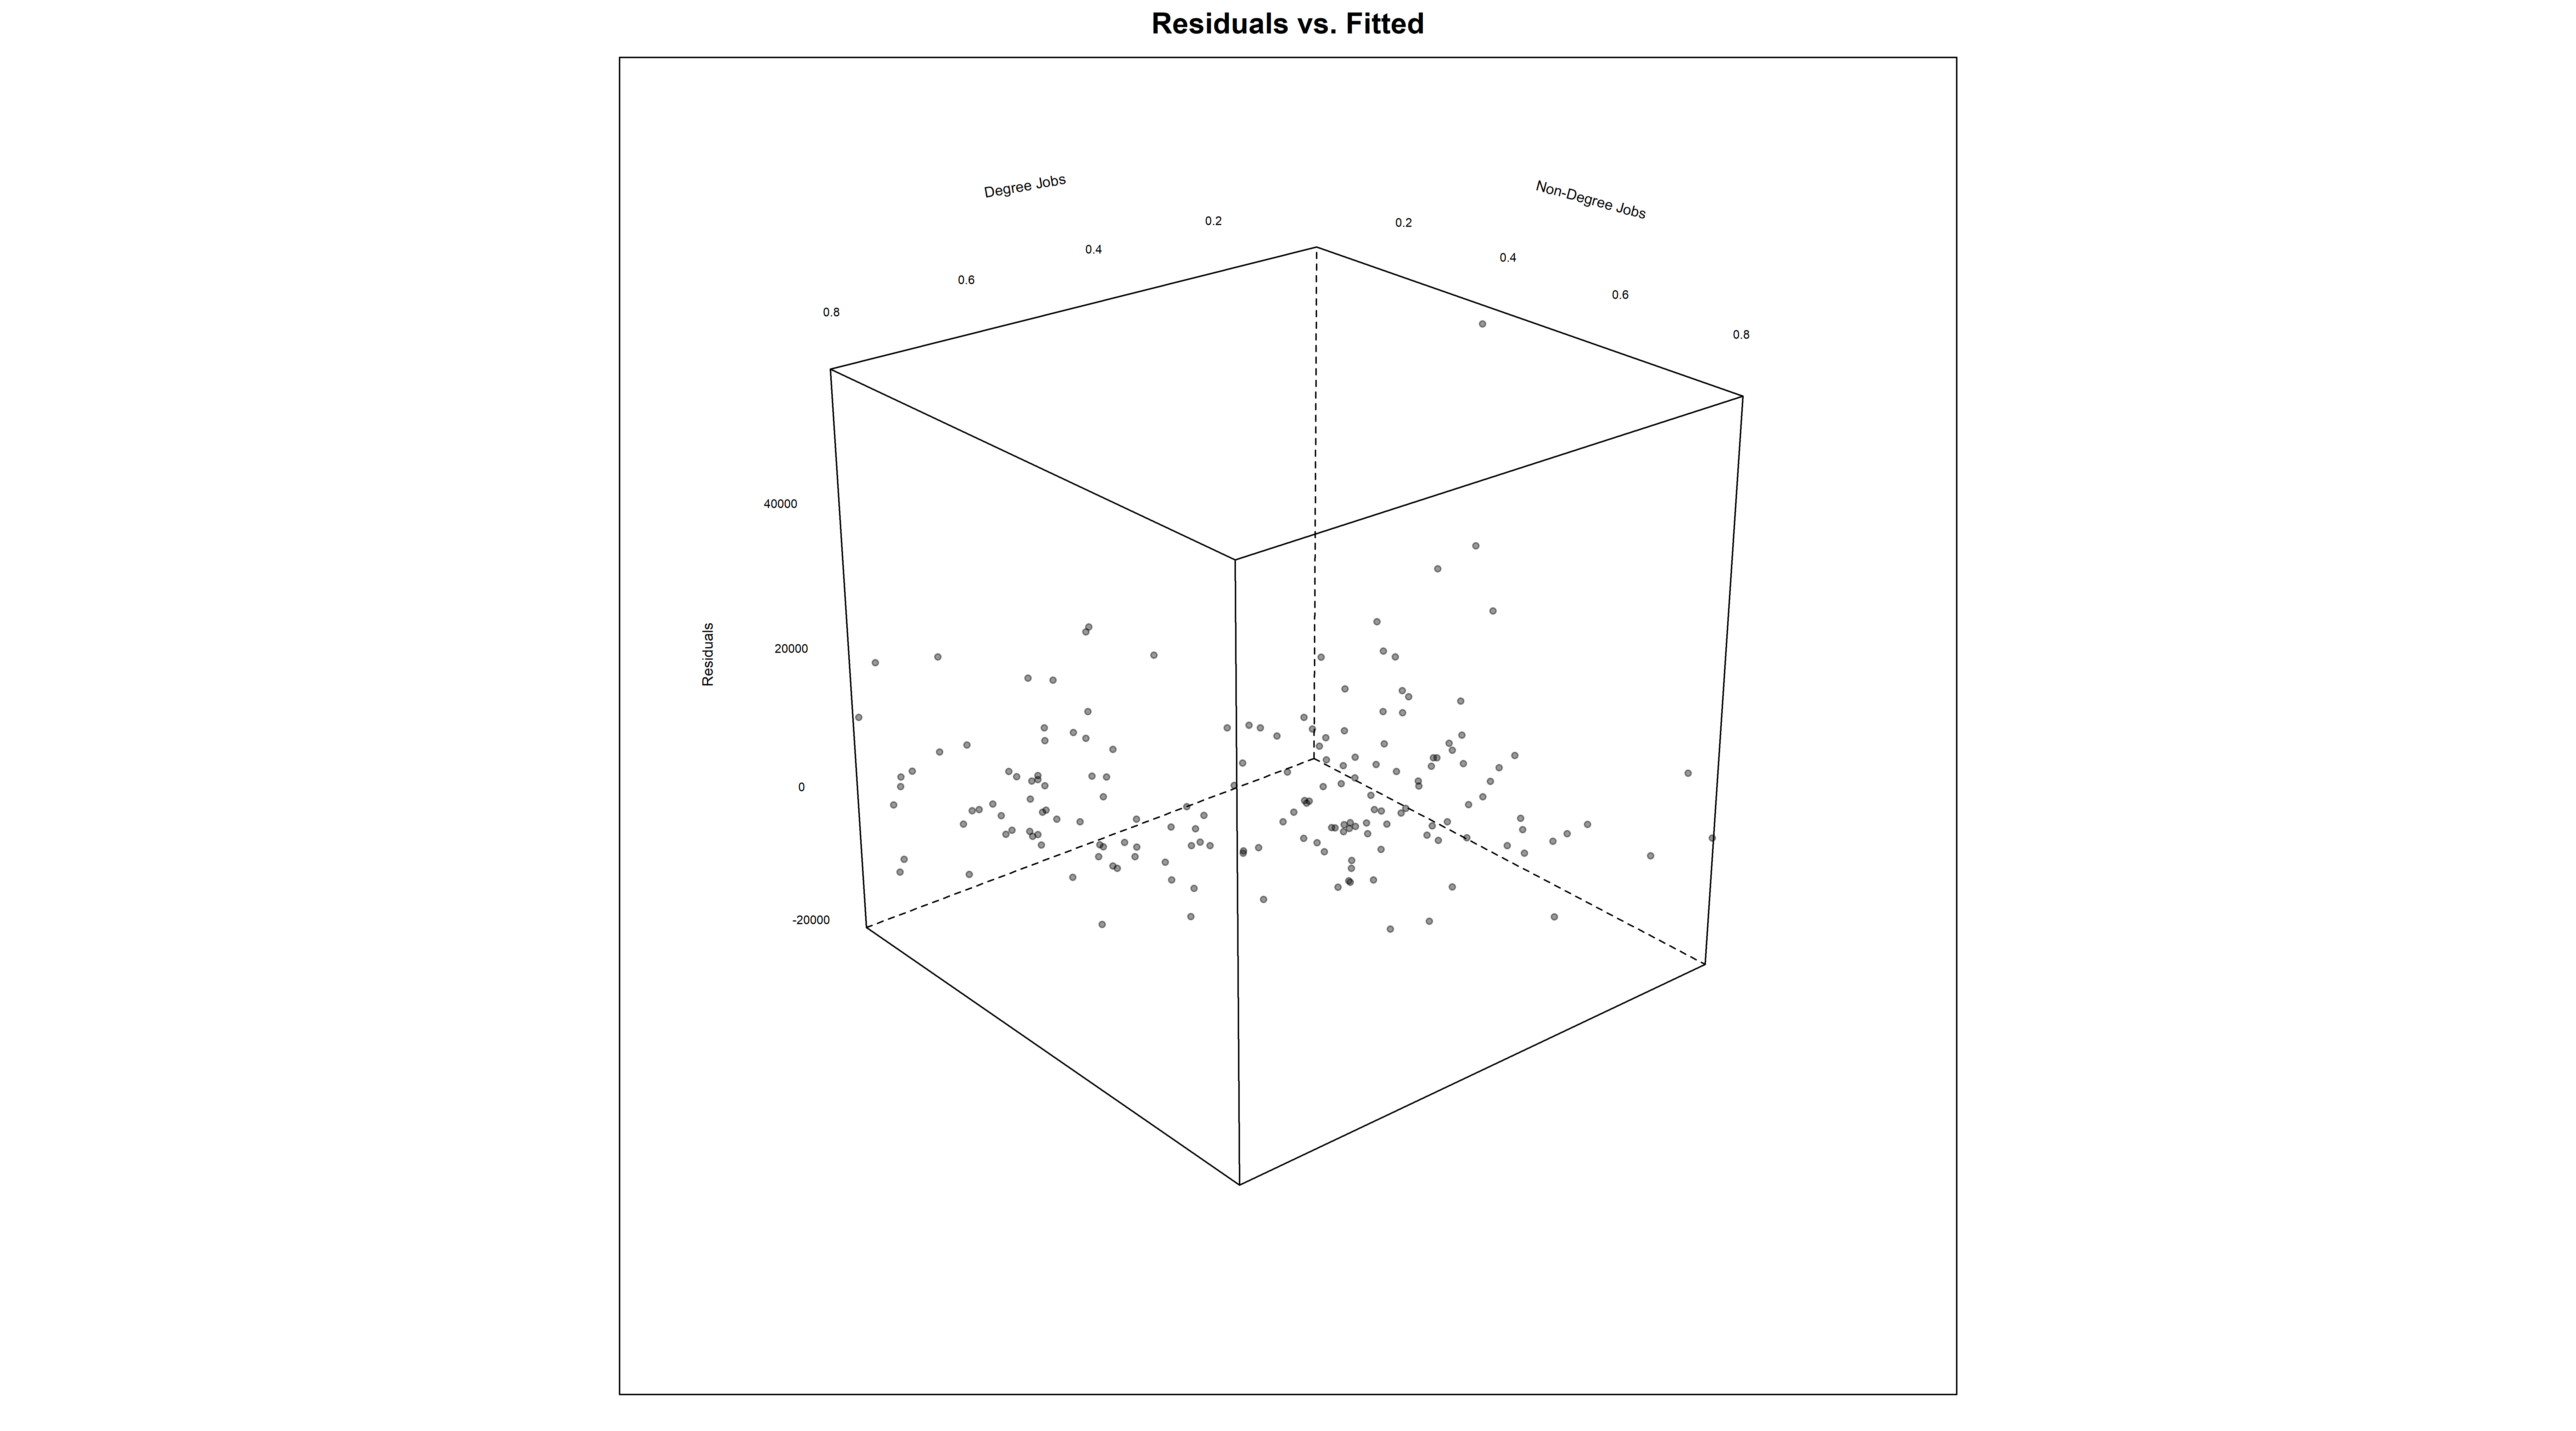
\includegraphics[scale=0.365]{plot2}
\caption{}
\end{figure}
%% -------------------------------------------------------------------------------------------|

%% [A-title] block ...
%% -------------------------------------------------------------------------------------------\
\begin{center}
\subsection{results}
\vspace{-3ex}
\end{center}
%% -------------------------------------------------------------------------------------------|

%% [B-paragraph] block ...
%% -------------------------------------------------------------------------------------------\
\noindent
A comparison of the results from the above procedure, with \textbf{r}'s built-in functions,
show that they are identical and that the above procedure is correct. Further, these
results reveal that a linear relation between the regressors and the response variables is
insignificant.
\smallskip
%% -------------------------------------------------------------------------------------------|

%% [C-code] block ...
%% -------------------------------------------------------------------------------------------\
\definecolor{lightgrey}{rgb}{0.972,0.972,0.972}
\begin{minted}[linenos=false, bgcolor=lightgrey, fontfamily=qcr, fontsize=\footnotesize]{r}
summary( lm(median ~ major_category + perc_college_jobs +
	    perc_non_college_jobs, data=df) )$coef # test for [linear relation] with t-test
\end{minted}
%% -------------------------------------------------------------------------------------------|

%% [D0-result-ctext] block ...
%% -------------------------------------------------------------------------------------------\
\definecolor{lightgrey}{rgb}{0.952,0.952,0.952}
\begin{minted}[linenos=false, bgcolor=lightgrey, fontfamily=qcr, fontsize=\footnotesize]{r}
                                                     Estimate Std. Error
(Intercept)                                        49602.2736   9030.389
major_categoryArts                                 -6341.6708   5418.893
major_categoryBiology & Life Science                -267.0807   4715.372
major_categoryBusiness                              4638.8226   4816.091
major_categoryCommunications & Journalism          -2088.8122   6723.287
major_categoryComputers & Mathematics              -9771.8766   5135.622
major_categoryEducation                            -5535.3195   4577.638
major_categoryEngineering                          -3472.6624   4177.666
major_categoryHealth                               -3802.9789   4882.036
major_categoryHumanities & Liberal Arts            -9685.5076   4697.485
major_categoryIndustrial Arts & Consumer Services  -3244.5961   5595.663
major_categoryInterdisciplinary                   -18801.7432  12183.909
major_categoryLaw & Public Policy                  -7089.2732   6273.079
major_categoryPhysical Sciences                    -3608.9103   5084.162
major_categoryPsychology & Social Work             -5585.4128   5334.146
major_categorySocial Science                       -4318.2703   5232.842
perc_college_jobs                                  -9849.5558   8728.567
perc_non_college_jobs                              -2473.7562  10848.308
                                                      t value     Pr(>|t|)
(Intercept)                                        5.49281690 1.600036e-07
major_categoryArts                                -1.17028901 2.436925e-01
major_categoryBiology & Life Science              -0.05664043 9.549050e-01
major_categoryBusiness                             0.96319248 3.369609e-01
major_categoryCommunications & Journalism         -0.31068316 7.564616e-01
major_categoryComputers & Mathematics             -1.90276400 5.893763e-02
major_categoryEducation                           -1.20920870 2.284358e-01
major_categoryEngineering                         -0.83124453 4.071225e-01
major_categoryHealth                              -0.77897389 4.371904e-01
major_categoryHumanities & Liberal Arts           -2.06184950 4.090272e-02
major_categoryIndustrial Arts & Consumer Services -0.57984119 5.628691e-01
major_categoryInterdisciplinary                   -1.54316186 1.248439e-01
major_categoryLaw & Public Policy                 -1.13011064 2.601867e-01
major_categoryPhysical Sciences                   -0.70983383 4.788806e-01
major_categoryPsychology & Social Work            -1.04710528 2.966917e-01
major_categorySocial Science                      -0.82522474 4.105205e-01
perc_college_jobs                                 -1.12842757 2.608943e-01
perc_non_college_jobs                             -0.22803152 8.199242e-01
\end{minted}
%% -------------------------------------------------------------------------------------------|

%% [C-code] block ...
%% -------------------------------------------------------------------------------------------\
\definecolor{lightgrey}{rgb}{0.972,0.972,0.972}
\begin{minted}[linenos=false, bgcolor=lightgrey, fontfamily=qcr, fontsize=\footnotesize]{r}
list(Y.values.vs.fitted=head(cbind(Y, Y_)),
     predictors=head(cbind(Z, X)),
     coefficients=cbind(GAMMA, SE.., t.B_, p_val.B_))$coefficients
\end{minted}
%% -------------------------------------------------------------------------------------------|

%% [D0-result-ctext] block ...
%% -------------------------------------------------------------------------------------------\
\definecolor{lightgrey}{rgb}{0.952,0.952,0.952}
\begin{minted}[linenos=false, bgcolor=lightgrey, fontfamily=qcr, fontsize=\footnotesize]{r}
                                                    Estimates Std. Error
(Intercept)                                        49602.2736   9030.389
major_categoryArts                                 -6341.6708   5418.893
major_categoryBiology & Life Science                -267.0807   4715.372
major_categoryBusiness                              4638.8226   4816.091
major_categoryCommunications & Journalism          -2088.8122   6723.287
major_categoryComputers & Mathematics              -9771.8766   5135.622
major_categoryEducation                            -5535.3195   4577.638
major_categoryEngineering                          -3472.6624   4177.666
major_categoryHealth                               -3802.9789   4882.036
major_categoryHumanities & Liberal Arts            -9685.5076   4697.485
major_categoryIndustrial Arts & Consumer Services  -3244.5961   5595.663
major_categoryInterdisciplinary                   -18801.7432  12183.909
major_categoryLaw & Public Policy                  -7089.2732   6273.079
major_categoryPhysical Sciences                    -3608.9103   5084.162
major_categoryPsychology & Social Work             -5585.4128   5334.146
major_categorySocial Science                       -4318.2703   5232.842
perc_college_jobs                                  -9849.5558   8728.567
perc_non_college_jobs                              -2473.7562  10848.308
                                                      t value     Pr(>|t|)
(Intercept)                                        5.49281690 1.600036e-07
major_categoryArts                                -1.17028901 2.436925e-01
major_categoryBiology & Life Science              -0.05664043 9.549050e-01
major_categoryBusiness                             0.96319248 3.369609e-01
major_categoryCommunications & Journalism         -0.31068316 7.564616e-01
major_categoryComputers & Mathematics             -1.90276400 5.893763e-02
major_categoryEducation                           -1.20920870 2.284358e-01
major_categoryEngineering                         -0.83124453 4.071225e-01
major_categoryHealth                              -0.77897389 4.371904e-01
major_categoryHumanities & Liberal Arts           -2.06184950 4.090272e-02
major_categoryIndustrial Arts & Consumer Services -0.57984119 5.628691e-01
major_categoryInterdisciplinary                   -1.54316186 1.248439e-01
major_categoryLaw & Public Policy                 -1.13011064 2.601867e-01
major_categoryPhysical Sciences                   -0.70983383 4.788806e-01
major_categoryPsychology & Social Work            -1.04710528 2.966917e-01
major_categorySocial Science                      -0.82522474 4.105205e-01
perc_college_jobs                                 -1.12842757 2.608943e-01
perc_non_college_jobs                             -0.22803152 8.199242e-01
\end{minted}
%% -------------------------------------------------------------------------------------------|

%% [C-code] block ...
%% -------------------------------------------------------------------------------------------\
\definecolor{lightgrey}{rgb}{0.972,0.972,0.972}
\begin{minted}[linenos=false, bgcolor=lightgrey, fontfamily=qcr, fontsize=\footnotesize]{r}
options(scipen = 999)
list(infl, inf.measures)
options(scipen = 0)
\end{minted}
%% -------------------------------------------------------------------------------------------|

%% [D0-result-ctext] block ...
%% -------------------------------------------------------------------------------------------\
\definecolor{lightgrey}{rgb}{0.952,0.952,0.952}
\begin{minted}[linenos=false, bgcolor=lightgrey, fontfamily=qcr, fontsize=\footnotesize]{r}
[[1]]
hii_LEVERAGE
   0.2209302

[[2]]
     yi      yi_        ei_         hii         ri_            Di_
1 33000 42216.23  -9216.231 0.012015861 -0.81692462 0.000427184315
2 58000 45641.31  12358.687 0.008332640  1.09343497 0.000528748242
3 40000 43851.68  -3851.682 0.006055751 -0.34038706 0.000037153395
4 65000 45094.40  19905.600 0.009234717  1.76194968 0.001522951989
5 45000 43943.40   1056.604 0.005921398  0.09336961 0.000002733135
6 31000 41124.02 -10124.018 0.026722668 -0.90414531 0.001181315954
\end{minted}
%% -------------------------------------------------------------------------------------------|

%% [B-paragraph] block ...
%% -------------------------------------------------------------------------------------------\
\noindent
Though there exists no linear relation in the model, that does not elimminate
other kinds of relations. Note that in \textsc{figure 2} the data seems to take
the form of either a \emph{stochastic} or \emph{sinusoidal} function. A new
question then arises, "why do median earnings appear volitle as the percentage of
jobs, requiring degrees and those that don't, increases?"
\smallskip
%% -------------------------------------------------------------------------------------------|

%% [D2-result-image] block ...
%% -------------------------------------------------------------------------------------------\
\begin{figure}[H]
\centering
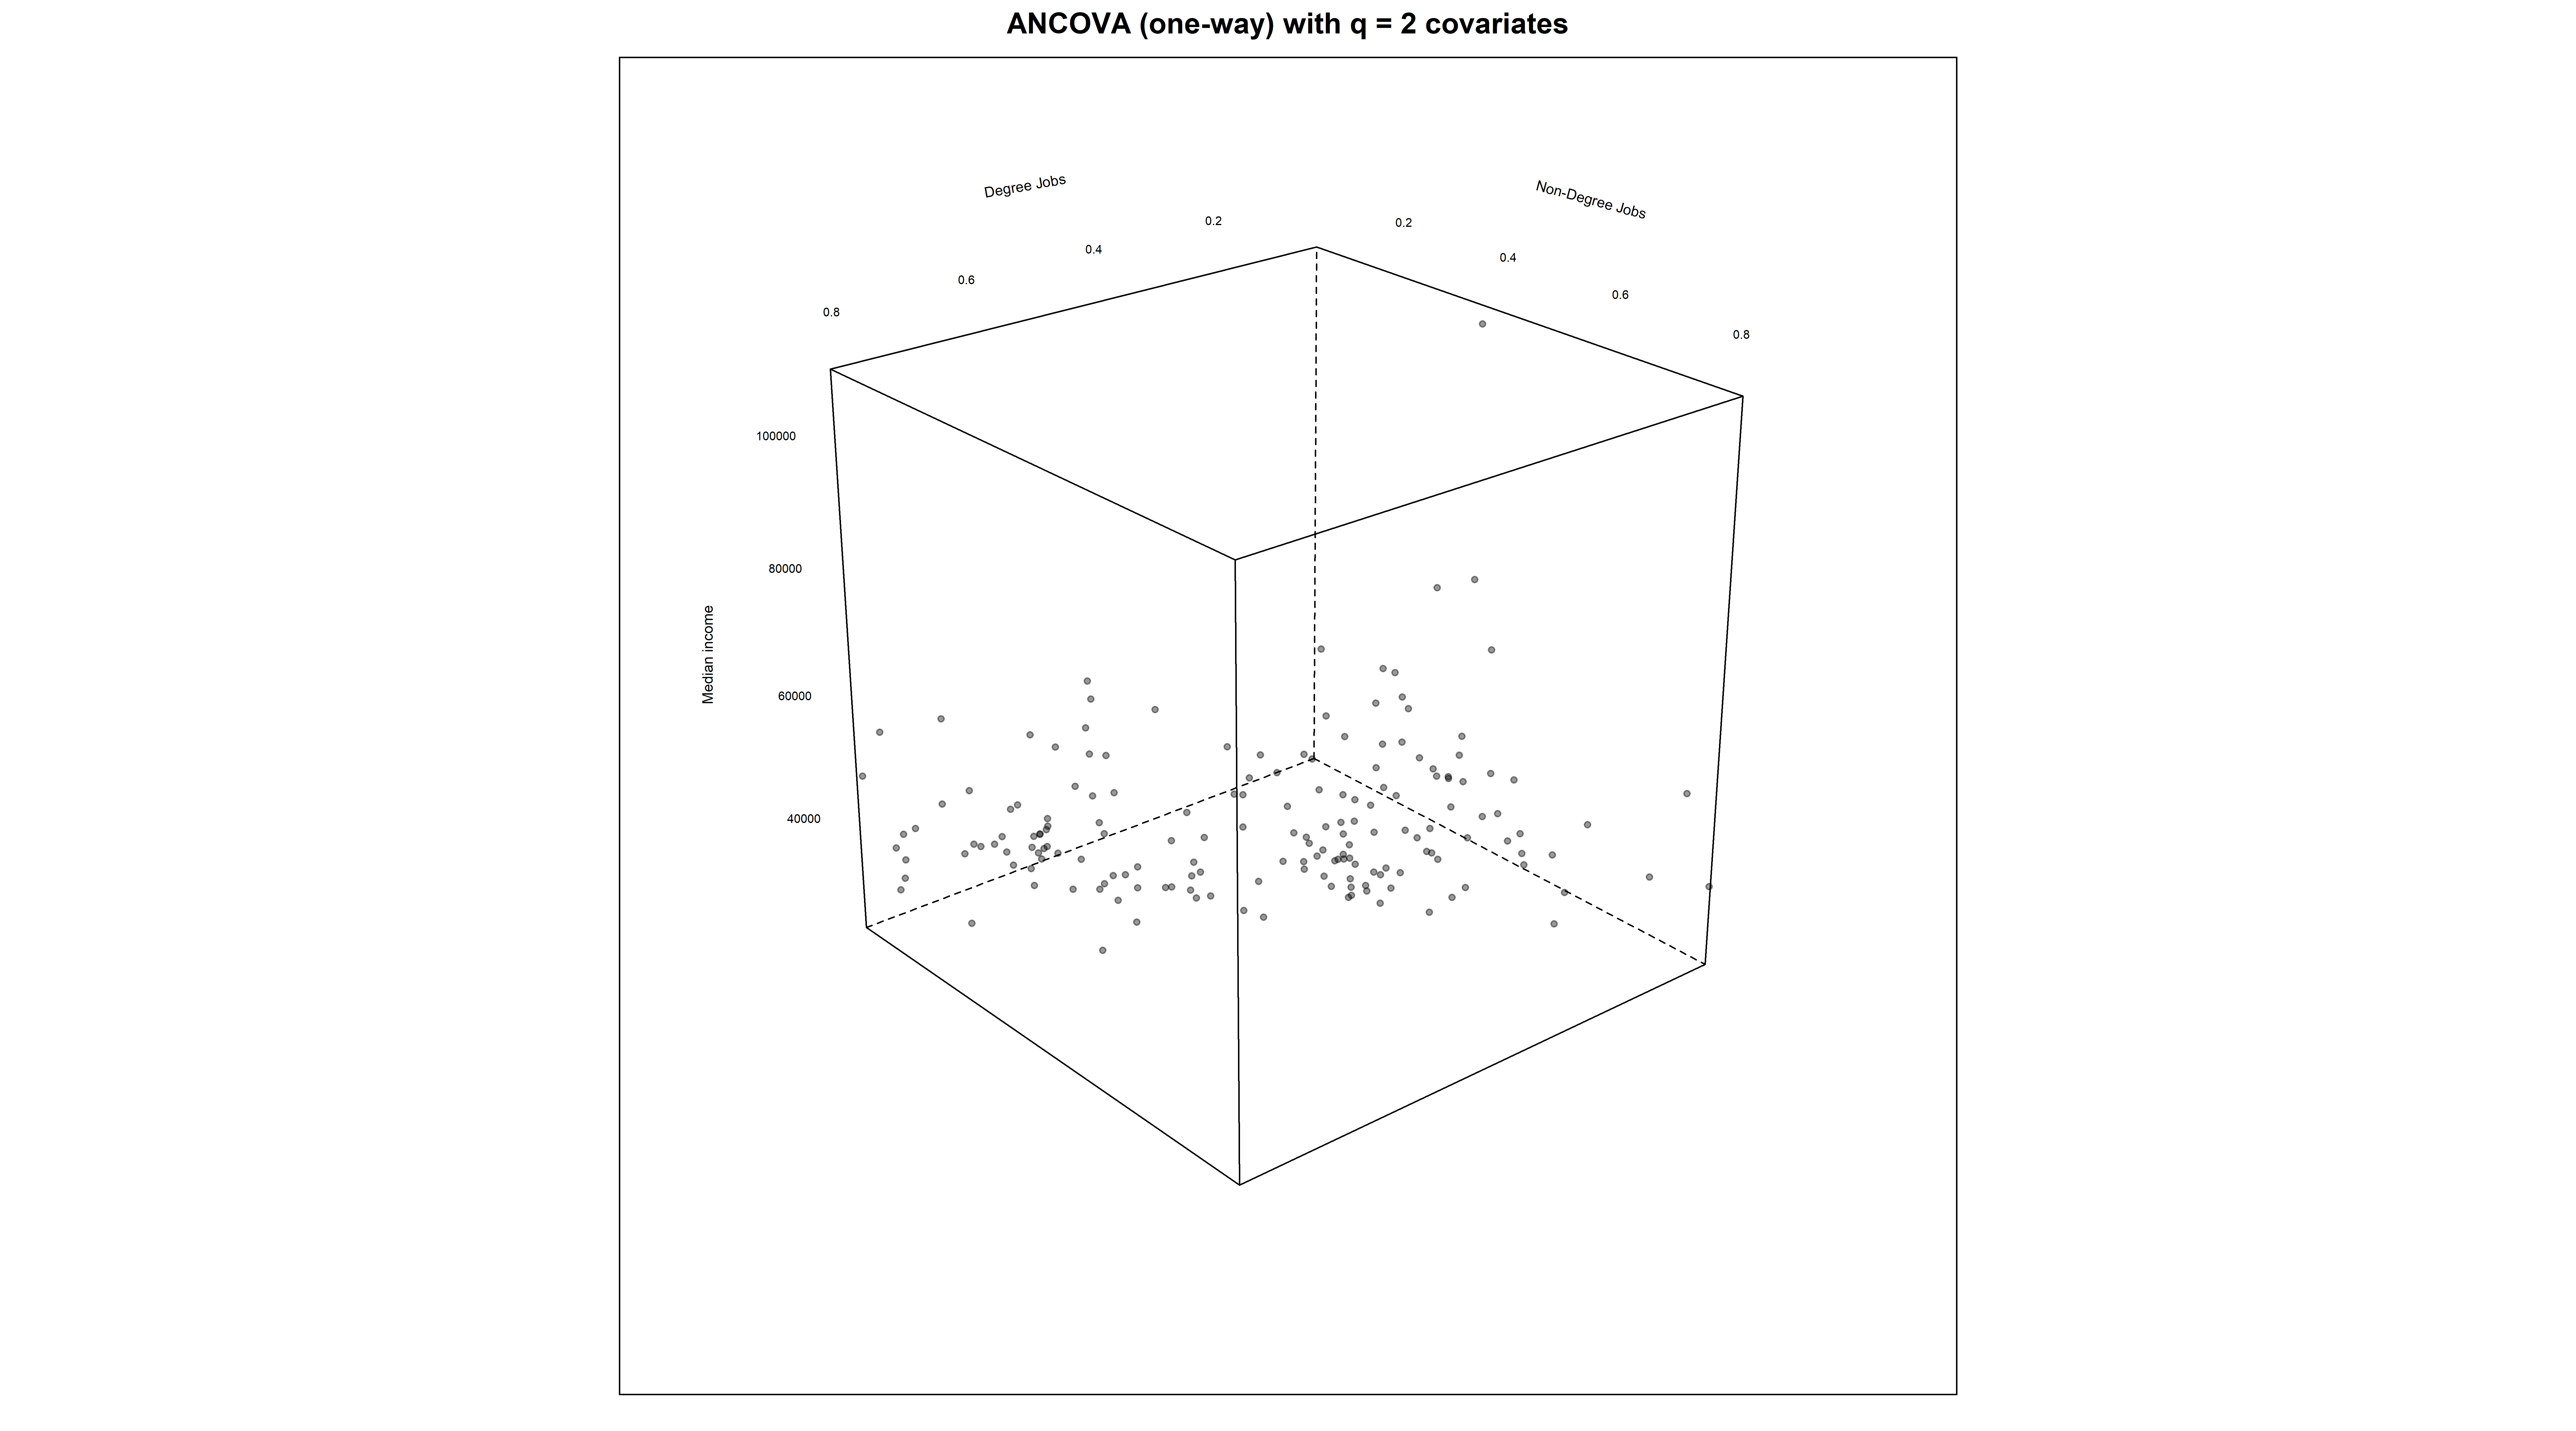
\includegraphics[scale=0.365]{plot1}
\caption{}
\end{figure}
%% -------------------------------------------------------------------------------------------|

%% [A-title] block ...
%% -------------------------------------------------------------------------------------------\
\begin{center}
\subsection{model validation}
\vspace{-3ex}
\end{center}
%% -------------------------------------------------------------------------------------------|

%% [B-paragraph] block ...
%% -------------------------------------------------------------------------------------------\
\noindent
Three new models are compared to determine which features are relevant and which are
irrelevant. To compare these models, use the \emph{vif} and \emph{anova} functions in \textbf{r}.
\smallskip
%% -------------------------------------------------------------------------------------------|

%% [C-code] block ...
%% -------------------------------------------------------------------------------------------\
\definecolor{lightgrey}{rgb}{0.972,0.972,0.972}
\begin{minted}[linenos=false, bgcolor=lightgrey, fontfamily=qcr, fontsize=\footnotesize]{r}
fit1 <- lm(median ~ major_category, data=df)
fit2 <- lm(median ~ major_category + perc_college_jobs, data=df)
fit3 <- lm(median ~ major_category + perc_college_jobs + perc_non_college_jobs, data=df)
anova(fit1, fit2, fit3)
\end{minted}
%% -------------------------------------------------------------------------------------------|

%% [D0-result-ctext] block ...
%% -------------------------------------------------------------------------------------------\
\definecolor{lightgrey}{rgb}{0.952,0.952,0.952}
\begin{minted}[linenos=false, bgcolor=lightgrey, fontfamily=qcr, fontsize=\footnotesize]{r}
Analysis of Variance Table

Model 1: median ~ major_category
Model 2: median ~ major_category + perc_college_jobs
Model 3: median ~ major_category + perc_college_jobs + perc_non_college_jobs
  Res.Df        RSS Df Sum of Sq      F Pr(>F)
1    156 2.0238e+10
2    155 1.9845e+10  1 392727096 3.0486 0.0828 .
3    154 1.9839e+10  1   6698576 0.0520 0.8199
---
Signif. codes:  0 '***' 0.001 '**' 0.01 '*' 0.05 '.' 0.1 ' ' 1
\end{minted}
%% -------------------------------------------------------------------------------------------|

%% [C-code] block ...
%% -------------------------------------------------------------------------------------------\
\definecolor{lightgrey}{rgb}{0.972,0.972,0.972}
\begin{minted}[linenos=false, bgcolor=lightgrey, fontfamily=qcr, fontsize=\footnotesize]{r}
fit4 <- aov(median ~ major_category + perc_college_jobs, data = df)
fit5 <- aov(median ~ major_category * perc_college_jobs, data = df)
anova(fit4, fit5)
\end{minted}
%% -------------------------------------------------------------------------------------------|

%% [D0-result-ctext] block ...
%% -------------------------------------------------------------------------------------------\
\definecolor{lightgrey}{rgb}{0.952,0.952,0.952}
\begin{minted}[linenos=false, bgcolor=lightgrey, fontfamily=qcr, fontsize=\footnotesize]{r}
Analysis of Variance Table

Model 1: median ~ major_category + perc_college_jobs
Model 2: median ~ major_category * perc_college_jobs
  Res.Df        RSS Df  Sum of Sq      F  Pr(>F)
1    155 1.9845e+10
2    141 1.6418e+10 14 3427295991 2.1024 0.01493 *
---
Signif. codes:  0 '***' 0.001 '**' 0.01 '*' 0.05 '.' 0.1 ' ' 1
\end{minted}
%% -------------------------------------------------------------------------------------------|

%% [C-code] block ...
%% -------------------------------------------------------------------------------------------\
\definecolor{lightgrey}{rgb}{0.972,0.972,0.972}
\begin{minted}[linenos=false, bgcolor=lightgrey, fontfamily=qcr, fontsize=\footnotesize]{r}
vif( lm(median ~ major_category + perc_college_jobs +
	         perc_non_college_jobs, data=df) ) # variance inflation factor
\end{minted}
%% -------------------------------------------------------------------------------------------|

%% [D0-result-ctext] block ...
%% -------------------------------------------------------------------------------------------\
\definecolor{lightgrey}{rgb}{0.952,0.952,0.952}
\begin{minted}[linenos=false, bgcolor=lightgrey, fontfamily=qcr, fontsize=\footnotesize]{r}
                          GVIF Df GVIF^(1/(2*Df))
major_category        1.260321 15        1.007742
perc_college_jobs     3.962138  1        1.990512
perc_non_college_jobs 3.876783  1        1.968955
\end{minted}
%% -------------------------------------------------------------------------------------------|

%% [B-paragraph] block ...
%% -------------------------------------------------------------------------------------------\
\noindent
The variance inflation factors for \textbf{per college jobs} and \textbf{perc non college jobs}
are moderately high, suggesting a removal of at least one of the two to get a more accurate model.
The adjusted model will now be explored in \textsc{case ii}.
\bigskip
%% -------------------------------------------------------------------------------------------|

%% ================ CASE 2 ====================================================================
%% [0-main] block ...
%% -------------------------------------------------------------------------------------------\
\begin{center}
\section{CASE II: POST-MODEL VALIDATION}
\vspace{-5ex}
\end{center}
%% -------------------------------------------------------------------------------------------|

%% [A-title] block ...
%% -------------------------------------------------------------------------------------------\
\begin{center}
\subsection{introduction}
\vspace{-3ex}
\end{center}
%% -------------------------------------------------------------------------------------------|

%% [B-paragraph] block ...
%% -------------------------------------------------------------------------------------------\
\noindent
I began my analysis by first constructing the ANCOVA model with all relevant features
that would assist in determining if there is truely an association between college
major category and income. However, after performing model validation, I removed
\textbf{perc non college jobs} from the model to get a more accurate result. I now explore
this adjusted model. 
\smallskip
%% -------------------------------------------------------------------------------------------|

%% [A-title] block ...
%% -------------------------------------------------------------------------------------------\
\begin{center}
\subsection{ancova one-way (unbalanced) model}
\vspace{-3ex}
\end{center}
%% -------------------------------------------------------------------------------------------|

%% [B-paragraph] block ...
%% -------------------------------------------------------------------------------------------\
\noindent
The ANCOVA (one-way) model will still bes used, but the covariates are now $q = 1$.
In mathematical notation, the model is expressed as
\begin{equation*}
\begin{aligned}
y_{ij} = \mu + \alpha_{i} + \beta x_{ij1} + \epsilon_{ij}
\end{aligned}
\end{equation*}
\smallskip

where:
\begin{equation*}
\begin{aligned}
& i = 1,2,...,k \ \text{observations}, \\
& j = 1,2,...,n \ \text{features}
\end{aligned}
\end{equation*}
\smallskip

\noindent
Here is the same model in matrix notation
\begin{equation*}
\begin{aligned}
\mathbf{y} = \mathbf{Z} \mathbf{\alpha} + \mathbf{X} \mathbf{\beta} + \mathbf{\epsilon}
\end{aligned}
\end{equation*}
\smallskip

where:
\begin{equation*}
\begin{aligned}
& \mathbf{Z} =
\left[ \begin{array}{ccccc}
    1 & 0 & 0 & \cdots & 0 \\
    \vdots & \vdots & \vdots &  & \vdots \\
    1 & 1 & 0 & \cdots & 0 \\
    1 & 1 & 0 & \cdots & 0 \\
    \vdots & \vdots & \vdots &  & \vdots \\
    1 & 0 & 0 & \cdots & 1, 
\end{array}\right]
, & \mathbf{\alpha} =
\left[ \begin{array}{c}
    \mu \\
    \alpha_{1}
\end{array}\right] \\
& & \\
& \mathbf{X} =
\left[ \begin{array}{ccccc}
    x_{111} \\
    x_{121} \\
    \vdots  \\
    x_{kn1}
\end{array}\right]
, & \mathbf{\beta} =
\left[ \begin{array}{c}
    \betahat_{1} 
\end{array}\right]
\end{aligned}
\end{equation*}
\smallskip

\noindent
$\mathbf{Z}$ is assumed to be rank-deficient and $\mathbf{X}$ is full-rank. As before,
$\mathbf{Z}$ will be reparameterized.
\smallskip
%% -------------------------------------------------------------------------------------------|

%% [C-code] block ...
%% -------------------------------------------------------------------------------------------\
\definecolor{lightgrey}{rgb}{0.972,0.972,0.972}
\begin{minted}[linenos=false, bgcolor=lightgrey, fontfamily=qcr, fontsize=\footnotesize]{r}
df <- college
df <- college %>% dplyr::select(median, major_category, perc_college_jobs)
df <- na.omit(df)
df <- arrange(df, major_category)
df[,2] <- as.factor(df[,2])
lapply(df, head)
df %>% group_by(major_category, .add=TRUE) %>% group_nest()
Z <- as.matrix( ( model.matrix( median ~ major_category, data=df) ) ) # full-rank
X <- as.matrix( cbind(df$perc_college_jobs) ) # full-rank
colnames(X) <- c("perc_college_jobs")
Y <- df$median
\end{minted}
%% -------------------------------------------------------------------------------------------|

%% [A-title] block ...
%% -------------------------------------------------------------------------------------------\
\begin{center}
\subsection{estimating parameters $\alpha$ \& $\beta$}
\vspace{-3ex}
\end{center}
%% -------------------------------------------------------------------------------------------|

%% [B-paragraph] block ...
%% -------------------------------------------------------------------------------------------\
\noindent
Calculations for parameters $\alphahat$ and $\betahat$ are the same as in \textsc{case i}
\smallskip

\begin{equation*}
\begin{aligned}
\alphahat = ( \mathbf{Z}^{'} \mathbf{Z} )^{-} ( \mathbf{Z}^{'} \mathbf{y} ) -
( \mathbf{Z}^{'} \mathbf{Z} )^{-} ( \mathbf{Z}^{'} \mathbf{X} \betahat )
\end{aligned}
\end{equation*}
\smallskip

\begin{equation*}
\begin{aligned}
\betahat & = ( \mathbf{X}^{'} \mathbf{Z} ) [ ( \mathbf{Z}^{'} \mathbf{Z})^{-}
( \mathbf{Z}^{'} \mathbf{y} ) - ( \mathbf{Z}^{'} \mathbf{Z} ) ( \mathbf{Z}^{'} \mathbf{X}
\betahat ) ] + \mathbf{X}^{'} \mathbf{X} \betahat = \mathbf{X}^{'} \mathbf{y} \\
	 & = ( \mathbf{X}^{'} \mathbf{Z} ) [ (\mathbf{Z}^{'} \mathbf{Z} )^{-}
( \mathbf{Z}^{'} \mathbf{y} ) ] - ( \mathbf{X}^{'} \mathbf{Z} )
[ ( \mathbf{Z}^{'} \mathbf{Z} )^{-} ( \mathbf{Z}^{'} \mathbf{X}
\betahat ) ] + \mathbf{X}^{'} \mathbf{X} \betahat = \mathbf{X}^{'} \mathbf{y} \\
	 & = \mathbf{X}^{'} [ \mathbf{Z} ( \mathbf{Z}^{'} \mathbf{Z} )^{-}
( \mathbf{Z}^{'} \mathbf{y} ) ] + \mathbf{X}^{'} [ \mathbf{I} - \mathbf{Z}
( \mathbf{Z}^{'} \mathbf{Z} )^{'} \mathbf{Z}^{'} ] \mathbf{X} \betahat = \mathbf{X}^{'} \mathbf{y} \\
	 & = \mathbf{X}^{'} ( \mathbf{P} ) \mathbf{y} + \mathbf{X}^{'} [ \mathbf{I} - \mathbf{P}]
\mathbf{X} \betahat = \mathbf{X}^{'} \mathbf{y} \\
	 & = \mathbf{X}^{'} [ \mathbf{I} - \mathbf{P} ] \mathbf{X} \betahat = \mathbf{X}^{'} \mathbf{y}
- \mathbf{X}^{'} ( \mathbf{P} ) \mathbf{y} \\
	 & = \mathbf{X}^{'} [ \mathbf{I} - \mathbf{P} ] \mathbf{X} \betahat = \mathbf{X}^{'}
[ \mathbf{I} - \mathbf{P} ] \mathbf{y} \\
	 & = \mathbf{E}_{xx}^{-} \mathbf{e}_{xy}
\end{aligned}
\end{equation*}
\smallskip

\noindent
A more compact form of the model can be expressed as
\begin{equation*}
\begin{aligned}
\mathbf{y} = \mathbf{U} \mathbf{\Gamma} + \mathbf{\epsilon}
\end{aligned}
\end{equation*}
\smallskip

where:
\begin{equation*}
\begin{aligned}
& \mathbf{U} =
\left[ \begin{array}{c}
    \mathbf{Z}, \ \mathbf{X}
\end{array}\right],
& \mathbf{\Gamma} =
\left[ \begin{array}{c}
    \alphahat \\
    \betahat
\end{array}\right]
\end{aligned}
\end{equation*}
\smallskip
%% -------------------------------------------------------------------------------------------|

%% [C-code] block ...
%% -------------------------------------------------------------------------------------------\
\definecolor{lightgrey}{rgb}{0.972,0.972,0.972}
\begin{minted}[linenos=false, bgcolor=lightgrey, fontfamily=qcr, fontsize=\footnotesize]{r}
P <- Z %*% ginv(t(Z) %*% Z) %*% t(Z)
I <- diag(dim(P)[1])
B_ <- solve(t(X) %*% (I - P) %*% X) %*% (t(X) %*% (I - P) %*% Y); colnames(B_) <- "Estimates"
A_ <- ginv(t(Z) %*% Z) %*% (t(Z) %*% Y) - ginv(t(Z) %*% Z) %*% (t(Z) %*% (X %*% B_))
rownames(A_) <- colnames(Z)
rownames(B_) <- colnames(X)
U <- cbind(Z, X)
GAMMA <- rbind(A_, B_)
Y_ <- U %*% GAMMA
\end{minted}
%% -------------------------------------------------------------------------------------------|

%% [A-title] block ...
%% -------------------------------------------------------------------------------------------\
\begin{center}
\subsection{degrees of freedom}
\vspace{-3ex}
\end{center}
%% -------------------------------------------------------------------------------------------|

%% [B-paragraph] block ...
%% -------------------------------------------------------------------------------------------\
\noindent
The degrees of freedom for the error term are the same as in \textsc{case i}. Therefore, $df = n - k$
\smallskip
%% -------------------------------------------------------------------------------------------|

%% [C-code] block ...
%% -------------------------------------------------------------------------------------------\
\definecolor{lightgrey}{rgb}{0.972,0.972,0.972}
\begin{minted}[linenos=false, bgcolor=lightgrey, fontfamily=qcr, fontsize=\footnotesize]{r}
n <- nrow(U); k <- qr(U)$rank
\end{minted}
%% -------------------------------------------------------------------------------------------|

%% [A-title] block ...
%% -------------------------------------------------------------------------------------------\
\begin{center}
\subsection{sum of squares}
\vspace{-3ex}
\end{center}
%% -------------------------------------------------------------------------------------------|

%% [B-paragraph] block ...
%% -------------------------------------------------------------------------------------------\
\noindent
Given the previous calculations, the \emph{sum of squares} can be calculated as such
\begin{equation*}
\begin{aligned}
SSE & = SS_{res} = \left( \mathbf{y} - \mathbf{\yhat} \right)^{'} \left( \mathbf{y} -
\mathbf{\yhat} \right) \\
SSR & = SS_{reg} = \left( \mathbf{y} - \mathbf{\ybar} \right)^{'} \left( \mathbf{y} -
\mathbf{\ybar} \right) \\
SST & = SS_{tot} = SS_{res} + SS_{reg} \\
R^{2} & = \frac{ SS_{res} }{ SS_{reg} } 
\end{aligned}
\end{equation*}
\smallskip
%% -------------------------------------------------------------------------------------------|

%% [C-code] block ...
%% -------------------------------------------------------------------------------------------\
\definecolor{lightgrey}{rgb}{0.972,0.972,0.972}
\begin{minted}[linenos=false, bgcolor=lightgrey, fontfamily=qcr, fontsize=\footnotesize]{r}
ss.res <- (t(Y) %*% Y) - (t(GAMMA) %*% t(U) %*% Y)
ss.reg <- t(Y_ - mean(Y)) %*% (Y_ - mean(Y))
ss.tot <- ss.res + ss.reg
R.2 <- ss.res/ss.reg
\end{minted}
%% -------------------------------------------------------------------------------------------|

%% [A-title] block ...
%% -------------------------------------------------------------------------------------------\
\begin{center}
\subsection{mean squares}
\vspace{-3ex}
\end{center}
%% -------------------------------------------------------------------------------------------|

%% [B-paragraph] block ...
%% -------------------------------------------------------------------------------------------\
\noindent
The sum of squared residuals, $SSE$ or $SS_{res}$ can be used to find the $MSE$
\begin{equation*}
\begin{aligned}
MSE & = \sigma^{2} \\
    & = \frac{ SS_{res} }{ k \left( n-1 \right) }
\end{aligned}
\end{equation*}
\smallskip

\noindent
Now the standard error of $\Gamma$, $SE_{\Gamma}$, can be found
\begin{equation*}
\begin{aligned}
SE_{\Gamma} = \sqrt{ diag(\sigma^{2} ( \mathbf{U}^{'} \mathbf{U})^{-} ) }
\end{aligned}
\end{equation*}
\smallskip
%% -------------------------------------------------------------------------------------------|

%% [C-code] block ...
%% -------------------------------------------------------------------------------------------\
\definecolor{lightgrey}{rgb}{0.972,0.972,0.972}
\begin{minted}[linenos=false, bgcolor=lightgrey, fontfamily=qcr, fontsize=\footnotesize]{r}
ms.res <- ss.res/(n-k)
SE.. <- matrix( sqrt( diag( ms.res[1] * solve(t(U) %*% U) ) ) );  colnames(SE..) <- "Std. Error"
\end{minted}
%% -------------------------------------------------------------------------------------------|

%% [A-title] block ...
%% -------------------------------------------------------------------------------------------\
\begin{center}
\subsection{hypothesis test}
\vspace{-3ex}
\end{center}
%% -------------------------------------------------------------------------------------------|

%% [B-paragraph] block ...
%% -------------------------------------------------------------------------------------------\
\noindent
A t-test is used to test for any such linear relation between the regressors and the
response variable.
\smallskip

\noindent
The hypothesis test and t-test are constructed below
\begin{equation*}
\begin{aligned}
& H_{0}: \Gamma = 0 \ \text{no linear relation.} \\
& H_{a}: \Gamma \neq 0 \ \text{linear relation exists.}
\end{aligned}
\end{equation*}
\smallskip

where:
\begin{equation*}
\begin{aligned}
\Gamma = 
\left[ \begin{array}{c}
    \alpha \\
    \beta_{1}
\end{array}\right]
\end{aligned}
\end{equation*}
\smallskip

\begin{equation*}
\begin{aligned}
t_{test} = \frac{ \Gamma - 0 }{ SE_{\Gamma} }
\end{aligned}
\end{equation*}
\smallskip

The null hypothesis, $H_{0}$, is rejected if $t_{test} \geq t_{1-\alpha, n-k}$. In \textsc{case i},
results from the t-test revealed no significant \emph{linear} relation between the regressors and
the response variable. Therefore, it can be assumed that this current t-test will also reach
the same conclusion, but with different results.
\smallskip
%% -------------------------------------------------------------------------------------------|

%% [C-code] block ...
%% -------------------------------------------------------------------------------------------\
\definecolor{lightgrey}{rgb}{0.972,0.972,0.972}
\begin{minted}[linenos=false, bgcolor=lightgrey, fontfamily=qcr, fontsize=\footnotesize]{r}
t.B_ <- GAMMA / SE..;  colnames(t.B_) <- "t value"
t.alpha <- qt(1-(0.05/2), df=n-k)
p_val.B_ <- 2*pt(-abs(t.B_), df=n-k);  colnames(p_val.B_) <- "Pr(>|t|)"
p_val.alpha <- 2*pt(-abs(t.alpha), df=n-k)
\end{minted}
%% -------------------------------------------------------------------------------------------|

%% [D0-result-ctext] block ...
%% -------------------------------------------------------------------------------------------\
\definecolor{lightgrey}{rgb}{0.952,0.952,0.952}
\begin{minted}[linenos=false, bgcolor=lightgrey, fontfamily=qcr, fontsize=\footnotesize]{r}
cbind(t.B_, p_val.B_)
                                                      t value     Pr(>|t|)
(Intercept)                                       11.01620338 3.296774e-21
major_categoryArts                                -1.15982207 2.479047e-01
major_categoryBiology & Life Science              -0.06175313 9.508390e-01
major_categoryBusiness                             0.98465353 3.263288e-01
major_categoryCommunications & Journalism         -0.31194760 7.554996e-01
major_categoryComputers & Mathematics             -1.92375132 5.621843e-02
major_categoryEducation                           -1.22078662 2.240207e-01
major_categoryEngineering                         -0.81882249 4.141448e-01
major_categoryHealth                              -0.79449323 4.281231e-01
major_categoryHumanities & Liberal Arts           -2.06100962 4.097298e-02
major_categoryIndustrial Arts & Consumer Services -0.58638810 5.584677e-01
major_categoryInterdisciplinary                   -1.53196755 1.275689e-01
major_categoryLaw & Public Policy                 -1.12162214 2.637577e-01
major_categoryPhysical Sciences                   -0.70927770 4.792177e-01
major_categoryPsychology & Social Work            -1.04421726 2.980107e-01
major_categorySocial Science                      -0.81217605 4.179362e-01
perc_college_jobs                                 -1.75138343 8.185791e-02
\end{minted}
%% -------------------------------------------------------------------------------------------|

%% [A-title] block ...
%% -------------------------------------------------------------------------------------------\
\begin{center}
\subsection{influencial observations and leverage}
\vspace{-3ex}
\end{center}
%% -------------------------------------------------------------------------------------------|

%% [B-paragraph] block ...
%% -------------------------------------------------------------------------------------------\
\noindent
It can be assumed, as in \textsc{case i}, that there exits no outliers whose presence
would have a huge impact on the model.
\smallskip
%% -------------------------------------------------------------------------------------------|

%% [C-code] block ...
%% -------------------------------------------------------------------------------------------\
\definecolor{lightgrey}{rgb}{0.972,0.972,0.972}
\begin{minted}[linenos=false, bgcolor=lightgrey, fontfamily=qcr, fontsize=\footnotesize]{r}
H <- X %*% solve(t(X) %*% X) %*% t(X)
create.hii <- function(mat=NULL)
{
	vec <- matrix(rep(0, nrow(mat)))
	for (i in 1:nrow(mat))
		for (j in 1:ncol(mat))
			if ( i == j)
				vec[i] <- mat[i,j] 
	vec
}
hii <- create.hii(mat=H) # leverage
e_ <- Y - Y_; # residual
r_ <- e_/sqrt(ms.res[1] * (1 - hii)) # studentized residual
D_ <- ((r_^2)/(k+1)) * ((hii)/(1-hii)) # Cook's distance
inf.measures <- cbind(head(Y), head(Y_), head(e_), head(hii), head(r_),  head(D_))
colnames(inf.measures) <- c("yi", "yi_", "ei_", "hii", "ri_", "Di_")
infl <- c( "hii_LEVERAGE"=(2*(k + 1))/n )
\end{minted}
%% -------------------------------------------------------------------------------------------|

%% [D0-result-ctext] block ...
%% -------------------------------------------------------------------------------------------\
\definecolor{lightgrey}{rgb}{0.952,0.952,0.952}
\begin{minted}[linenos=false, bgcolor=lightgrey, fontfamily=qcr, fontsize=\footnotesize]{r}
list(infl, inf.measures)

[[1]]
hii_LEVERAGE
   0.2209302

[[2]]
     yi      yi_        ei_         hii         ri_          Di_
1 33000 42216.23  -9216.231 0.012015861 -0.81692462 4.271843e-04
2 58000 45641.31  12358.687 0.008332640  1.09343497 5.287482e-04
3 40000 43851.68  -3851.682 0.006055751 -0.34038706 3.715339e-05
4 65000 45094.40  19905.600 0.009234717  1.76194968 1.522952e-03
5 45000 43943.40   1056.604 0.005921398  0.09336961 2.733135e-06
6 31000 41124.02 -10124.018 0.026722668 -0.90414531 1.181316e-03
\end{minted}
%% -------------------------------------------------------------------------------------------|

%% [D2-result-image] block ...
%% -------------------------------------------------------------------------------------------\
\begin{figure}[H]
\centering
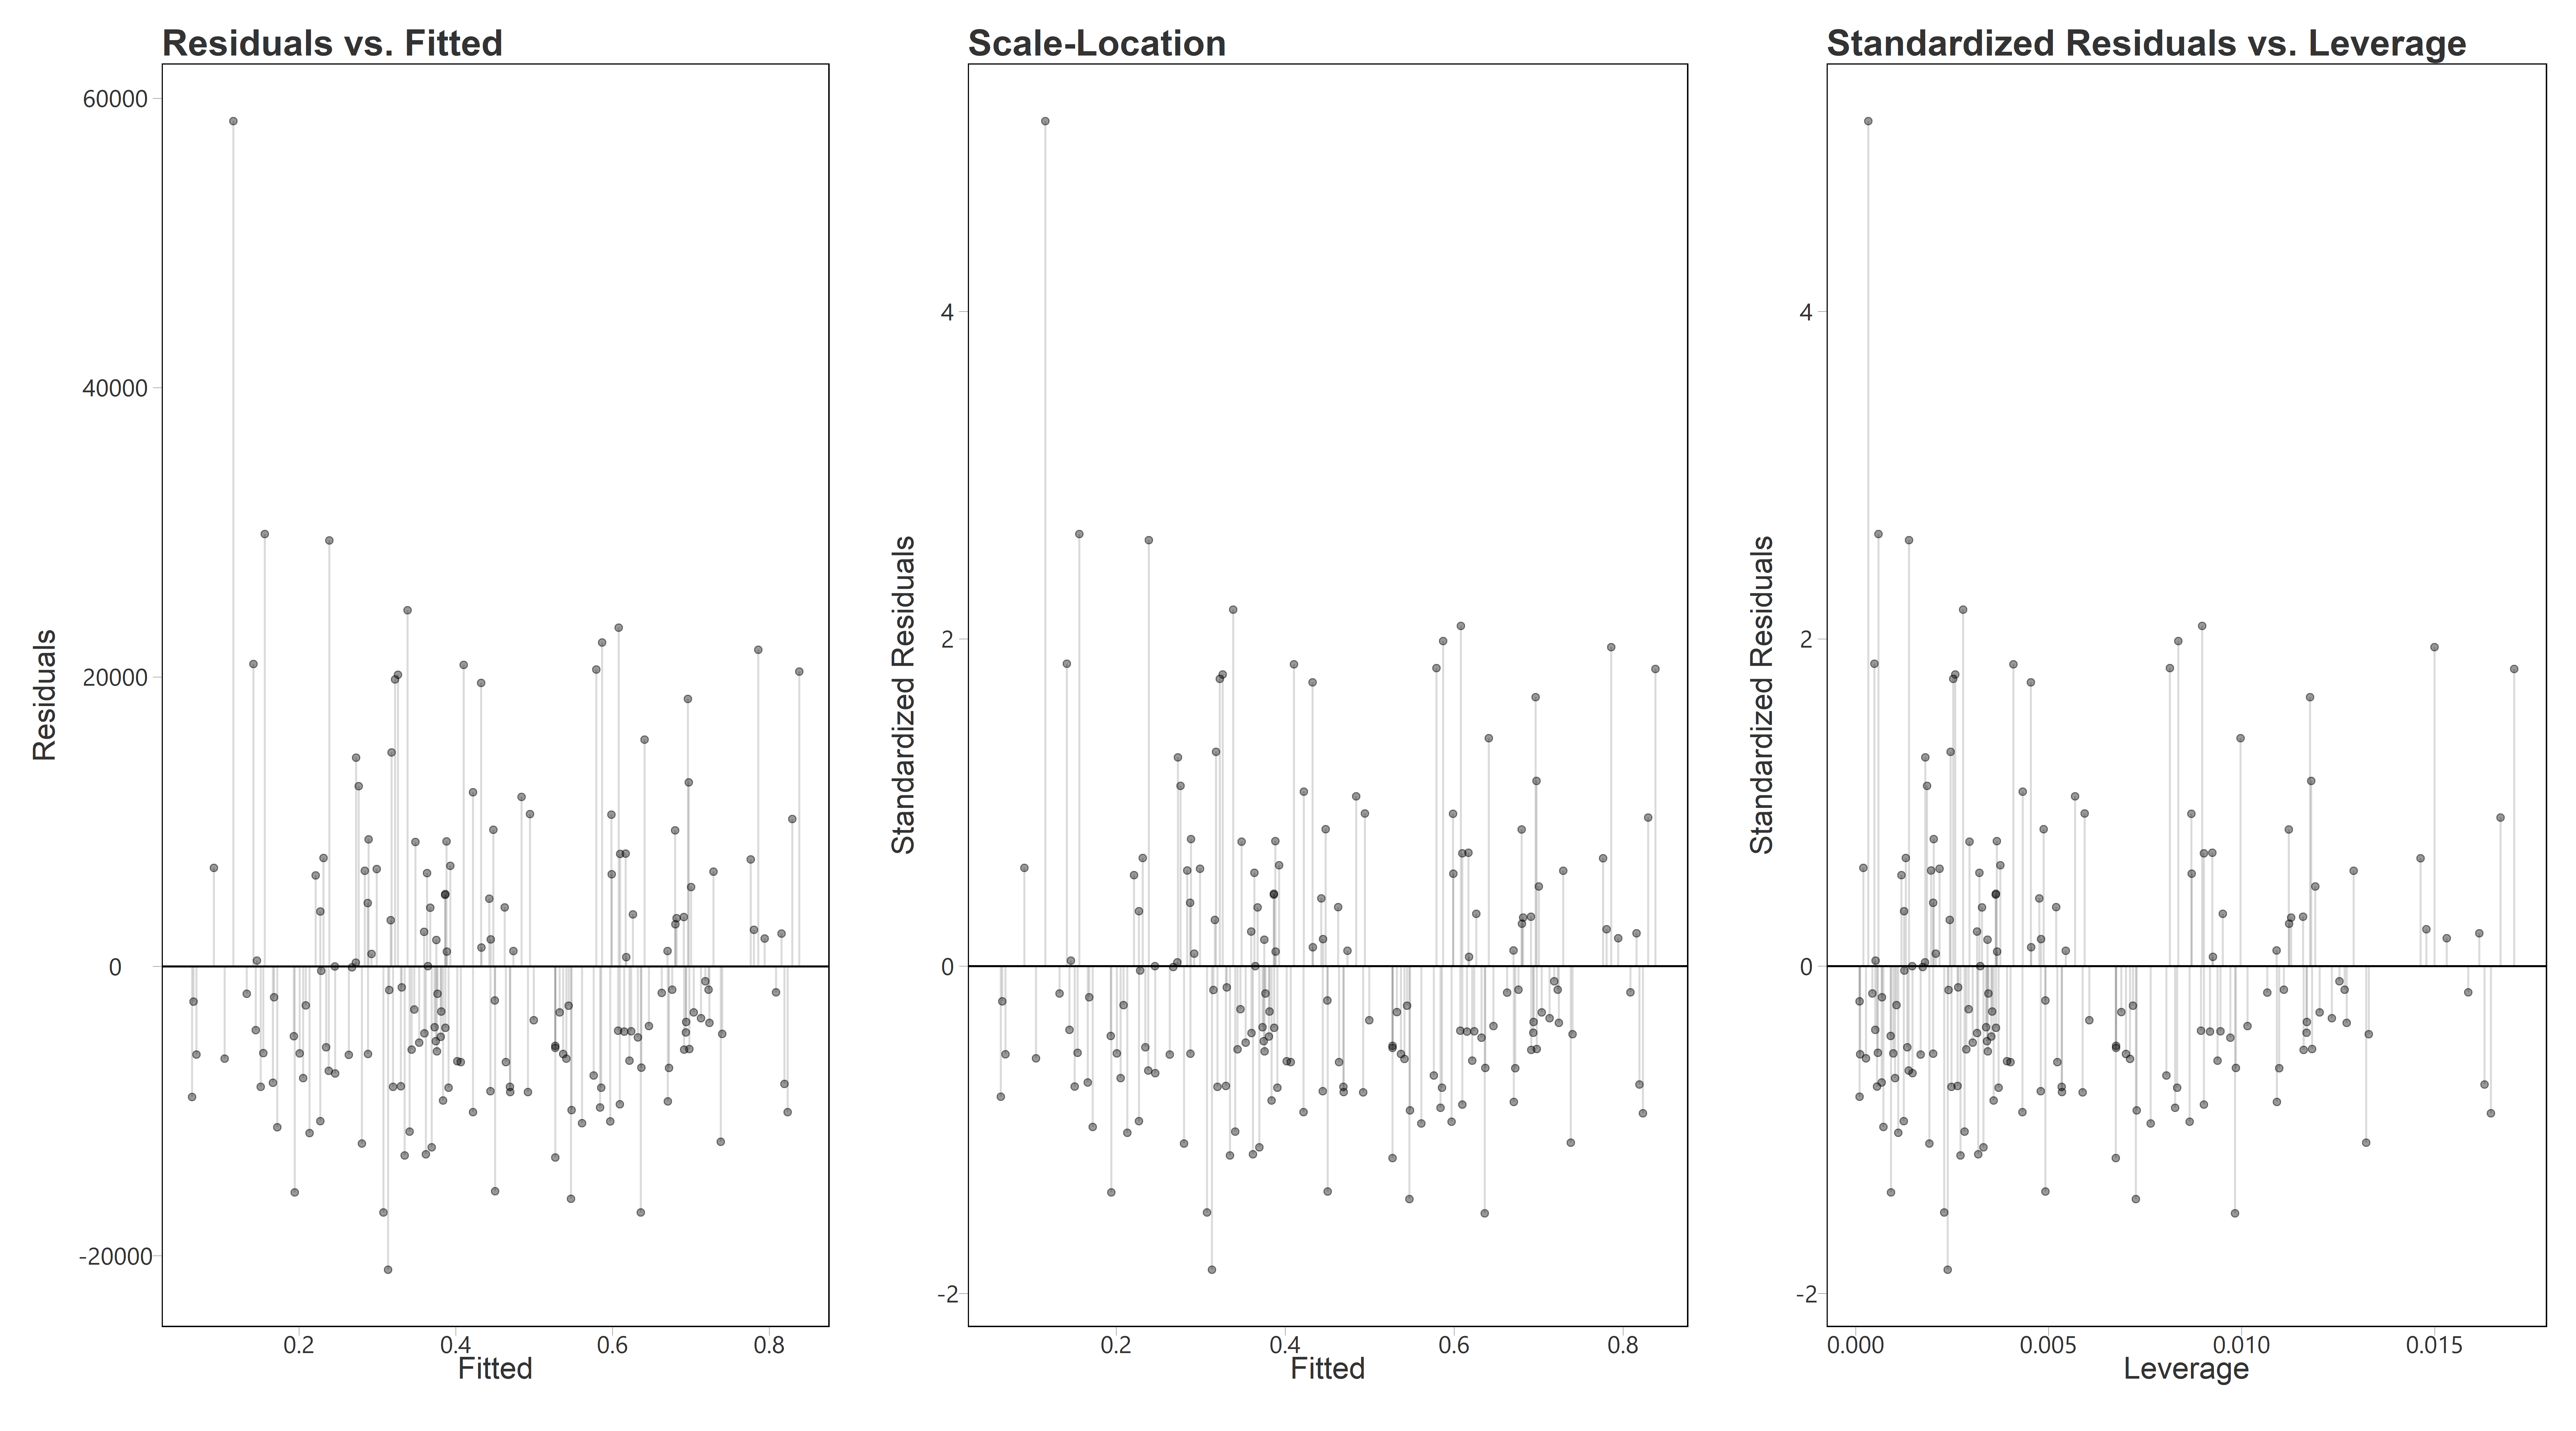
\includegraphics[scale=0.365]{plot3}
\caption{}
\end{figure}
%% -------------------------------------------------------------------------------------------|

%% [A-title] block ...
%% -------------------------------------------------------------------------------------------\
\begin{center}
\subsection{results}
\vspace{-3ex}
\end{center}
%% -------------------------------------------------------------------------------------------|

%% [B-paragraph] block ...
%% -------------------------------------------------------------------------------------------\
\noindent
Again, results show very low signs of linearity between the regressors and the response
variable. More sophisticated mathematical modeling techniques will be needed for
discovering the \textbf{proper} relation between the regressors and response variable.
\smallskip
%% -------------------------------------------------------------------------------------------|

%% [C-code] block ...
%% -------------------------------------------------------------------------------------------\
\definecolor{lightgrey}{rgb}{0.972,0.972,0.972}
\begin{minted}[linenos=false, bgcolor=lightgrey, fontfamily=qcr, fontsize=\footnotesize]{r}
summary( lm(median ~ major_category + perc_college_jobs, data=df) )$coef
\end{minted}
%% -------------------------------------------------------------------------------------------|

%% [D0-result-ctext] block ...
%% -------------------------------------------------------------------------------------------\
\definecolor{lightgrey}{rgb}{0.952,0.952,0.952}
\begin{minted}[linenos=false, bgcolor=lightgrey, fontfamily=qcr, fontsize=\footnotesize]{r}
                                                     Estimate Std. Error
(Intercept)                                        47797.9954   4338.881
major_categoryArts                                 -6247.4680   5386.575
major_categoryBiology & Life Science                -290.2299   4699.841
major_categoryBusiness                              4715.9758   4789.477
major_categoryCommunications & Journalism          -2090.8879   6702.689
major_categoryComputers & Mathematics              -9835.0563   5112.436
major_categoryEducation                            -5568.4043   4561.325
major_categoryEngineering                          -3400.4889   4152.901
major_categoryHealth                               -3861.5159   4860.351
major_categoryHumanities & Liberal Arts            -9645.0093   4679.750
major_categoryIndustrial Arts & Consumer Services  -3270.5064   5577.375
major_categoryInterdisciplinary                   -18290.7687  11939.397
major_categoryLaw & Public Policy                  -7001.1519   6241.988
major_categoryPhysical Sciences                    -3594.7709   5068.214
major_categoryPsychology & Social Work             -5550.6843   5315.641
major_categorySocial Science                       -4223.6223   5200.378
perc_college_jobs                                  -8169.2759   4664.470
                                                      t value     Pr(>|t|)
(Intercept)                                       11.01620338 3.296774e-21
major_categoryArts                                -1.15982207 2.479047e-01
major_categoryBiology & Life Science              -0.06175313 9.508390e-01
major_categoryBusiness                             0.98465353 3.263288e-01
major_categoryCommunications & Journalism         -0.31194760 7.554996e-01
major_categoryComputers & Mathematics             -1.92375132 5.621843e-02
major_categoryEducation                           -1.22078662 2.240207e-01
major_categoryEngineering                         -0.81882249 4.141448e-01
major_categoryHealth                              -0.79449323 4.281231e-01
major_categoryHumanities & Liberal Arts           -2.06100962 4.097298e-02
major_categoryIndustrial Arts & Consumer Services -0.58638810 5.584677e-01
major_categoryInterdisciplinary                   -1.53196755 1.275689e-01
major_categoryLaw & Public Policy                 -1.12162214 2.637577e-01
major_categoryPhysical Sciences                   -0.70927770 4.792177e-01
major_categoryPsychology & Social Work            -1.04421726 2.980107e-01
major_categorySocial Science                      -0.81217605 4.179362e-01
perc_college_jobs                                 -1.75138343 8.185791e-02
\end{minted}
%% -------------------------------------------------------------------------------------------|

%% [C-code] block ...
%% -------------------------------------------------------------------------------------------\
\definecolor{lightgrey}{rgb}{0.972,0.972,0.972}
\begin{minted}[linenos=false, bgcolor=lightgrey, fontfamily=qcr, fontsize=\footnotesize]{r}
list(Y.values.vs.fitted=head(cbind(Y, Y_)), predictors=head(cbind(Z, X)),
     coefficients=cbind(GAMMA, SE.., t.B_, p_val.B_))$coefficients
\end{minted}
%% -------------------------------------------------------------------------------------------|

%% [D0-result-ctext] block ...
%% -------------------------------------------------------------------------------------------\
\definecolor{lightgrey}{rgb}{0.952,0.952,0.952}
\begin{minted}[linenos=false, bgcolor=lightgrey, fontfamily=qcr, fontsize=\footnotesize]{r}
                                                    Estimates Std. Error
(Intercept)                                        47797.9954   4338.881
major_categoryArts                                 -6247.4680   5386.575
major_categoryBiology & Life Science                -290.2299   4699.841
major_categoryBusiness                              4715.9758   4789.477
major_categoryCommunications & Journalism          -2090.8879   6702.689
major_categoryComputers & Mathematics              -9835.0563   5112.436
major_categoryEducation                            -5568.4043   4561.325
major_categoryEngineering                          -3400.4889   4152.901
major_categoryHealth                               -3861.5159   4860.351
major_categoryHumanities & Liberal Arts            -9645.0093   4679.750
major_categoryIndustrial Arts & Consumer Services  -3270.5064   5577.375
major_categoryInterdisciplinary                   -18290.7687  11939.397
major_categoryLaw & Public Policy                  -7001.1519   6241.988
major_categoryPhysical Sciences                    -3594.7709   5068.214
major_categoryPsychology & Social Work             -5550.6843   5315.641
major_categorySocial Science                       -4223.6223   5200.378
perc_college_jobs                                  -8169.2759   4664.470
                                                      t value     Pr(>|t|)
(Intercept)                                       11.01620338 3.296774e-21
major_categoryArts                                -1.15982207 2.479047e-01
major_categoryBiology & Life Science              -0.06175313 9.508390e-01
major_categoryBusiness                             0.98465353 3.263288e-01
major_categoryCommunications & Journalism         -0.31194760 7.554996e-01
major_categoryComputers & Mathematics             -1.92375132 5.621843e-02
major_categoryEducation                           -1.22078662 2.240207e-01
major_categoryEngineering                         -0.81882249 4.141448e-01
major_categoryHealth                              -0.79449323 4.281231e-01
major_categoryHumanities & Liberal Arts           -2.06100962 4.097298e-02
major_categoryIndustrial Arts & Consumer Services -0.58638810 5.584677e-01
major_categoryInterdisciplinary                   -1.53196755 1.275689e-01
major_categoryLaw & Public Policy                 -1.12162214 2.637577e-01
major_categoryPhysical Sciences                   -0.70927770 4.792177e-01
major_categoryPsychology & Social Work            -1.04421726 2.980107e-01
major_categorySocial Science                      -0.81217605 4.179362e-01
perc_college_jobs                                 -1.75138343 8.185791e-02
\end{minted}
%% -------------------------------------------------------------------------------------------|

%% [C-code] block ...
%% -------------------------------------------------------------------------------------------\
\definecolor{lightgrey}{rgb}{0.972,0.972,0.972}
\begin{minted}[linenos=false, bgcolor=lightgrey, fontfamily=qcr, fontsize=\footnotesize]{r}
options(scipen = 999)
list(infl, inf.measures)
options(scipen = 0)
\end{minted}
%% -------------------------------------------------------------------------------------------|

%% [D0-result-ctext] block ...
%% -------------------------------------------------------------------------------------------\
\definecolor{lightgrey}{rgb}{0.952,0.952,0.952}
\begin{minted}[linenos=false, bgcolor=lightgrey, fontfamily=qcr, fontsize=\footnotesize]{r}
[[1]]
hii_LEVERAGE
   0.2209302

[[2]]
     yi      yi_        ei_         hii         ri_            Di_
1 33000 42216.23  -9216.231 0.012015861 -0.81692462 0.000427184315
2 58000 45641.31  12358.687 0.008332640  1.09343497 0.000528748242
3 40000 43851.68  -3851.682 0.006055751 -0.34038706 0.000037153395
4 65000 45094.40  19905.600 0.009234717  1.76194968 0.001522951989
5 45000 43943.40   1056.604 0.005921398  0.09336961 0.000002733135
6 31000 41124.02 -10124.018 0.026722668 -0.90414531 0.001181315954
\end{minted}
%% -------------------------------------------------------------------------------------------|

%% [D2-result-image] block ...
%% -------------------------------------------------------------------------------------------\
\begin{figure}[H]
\centering
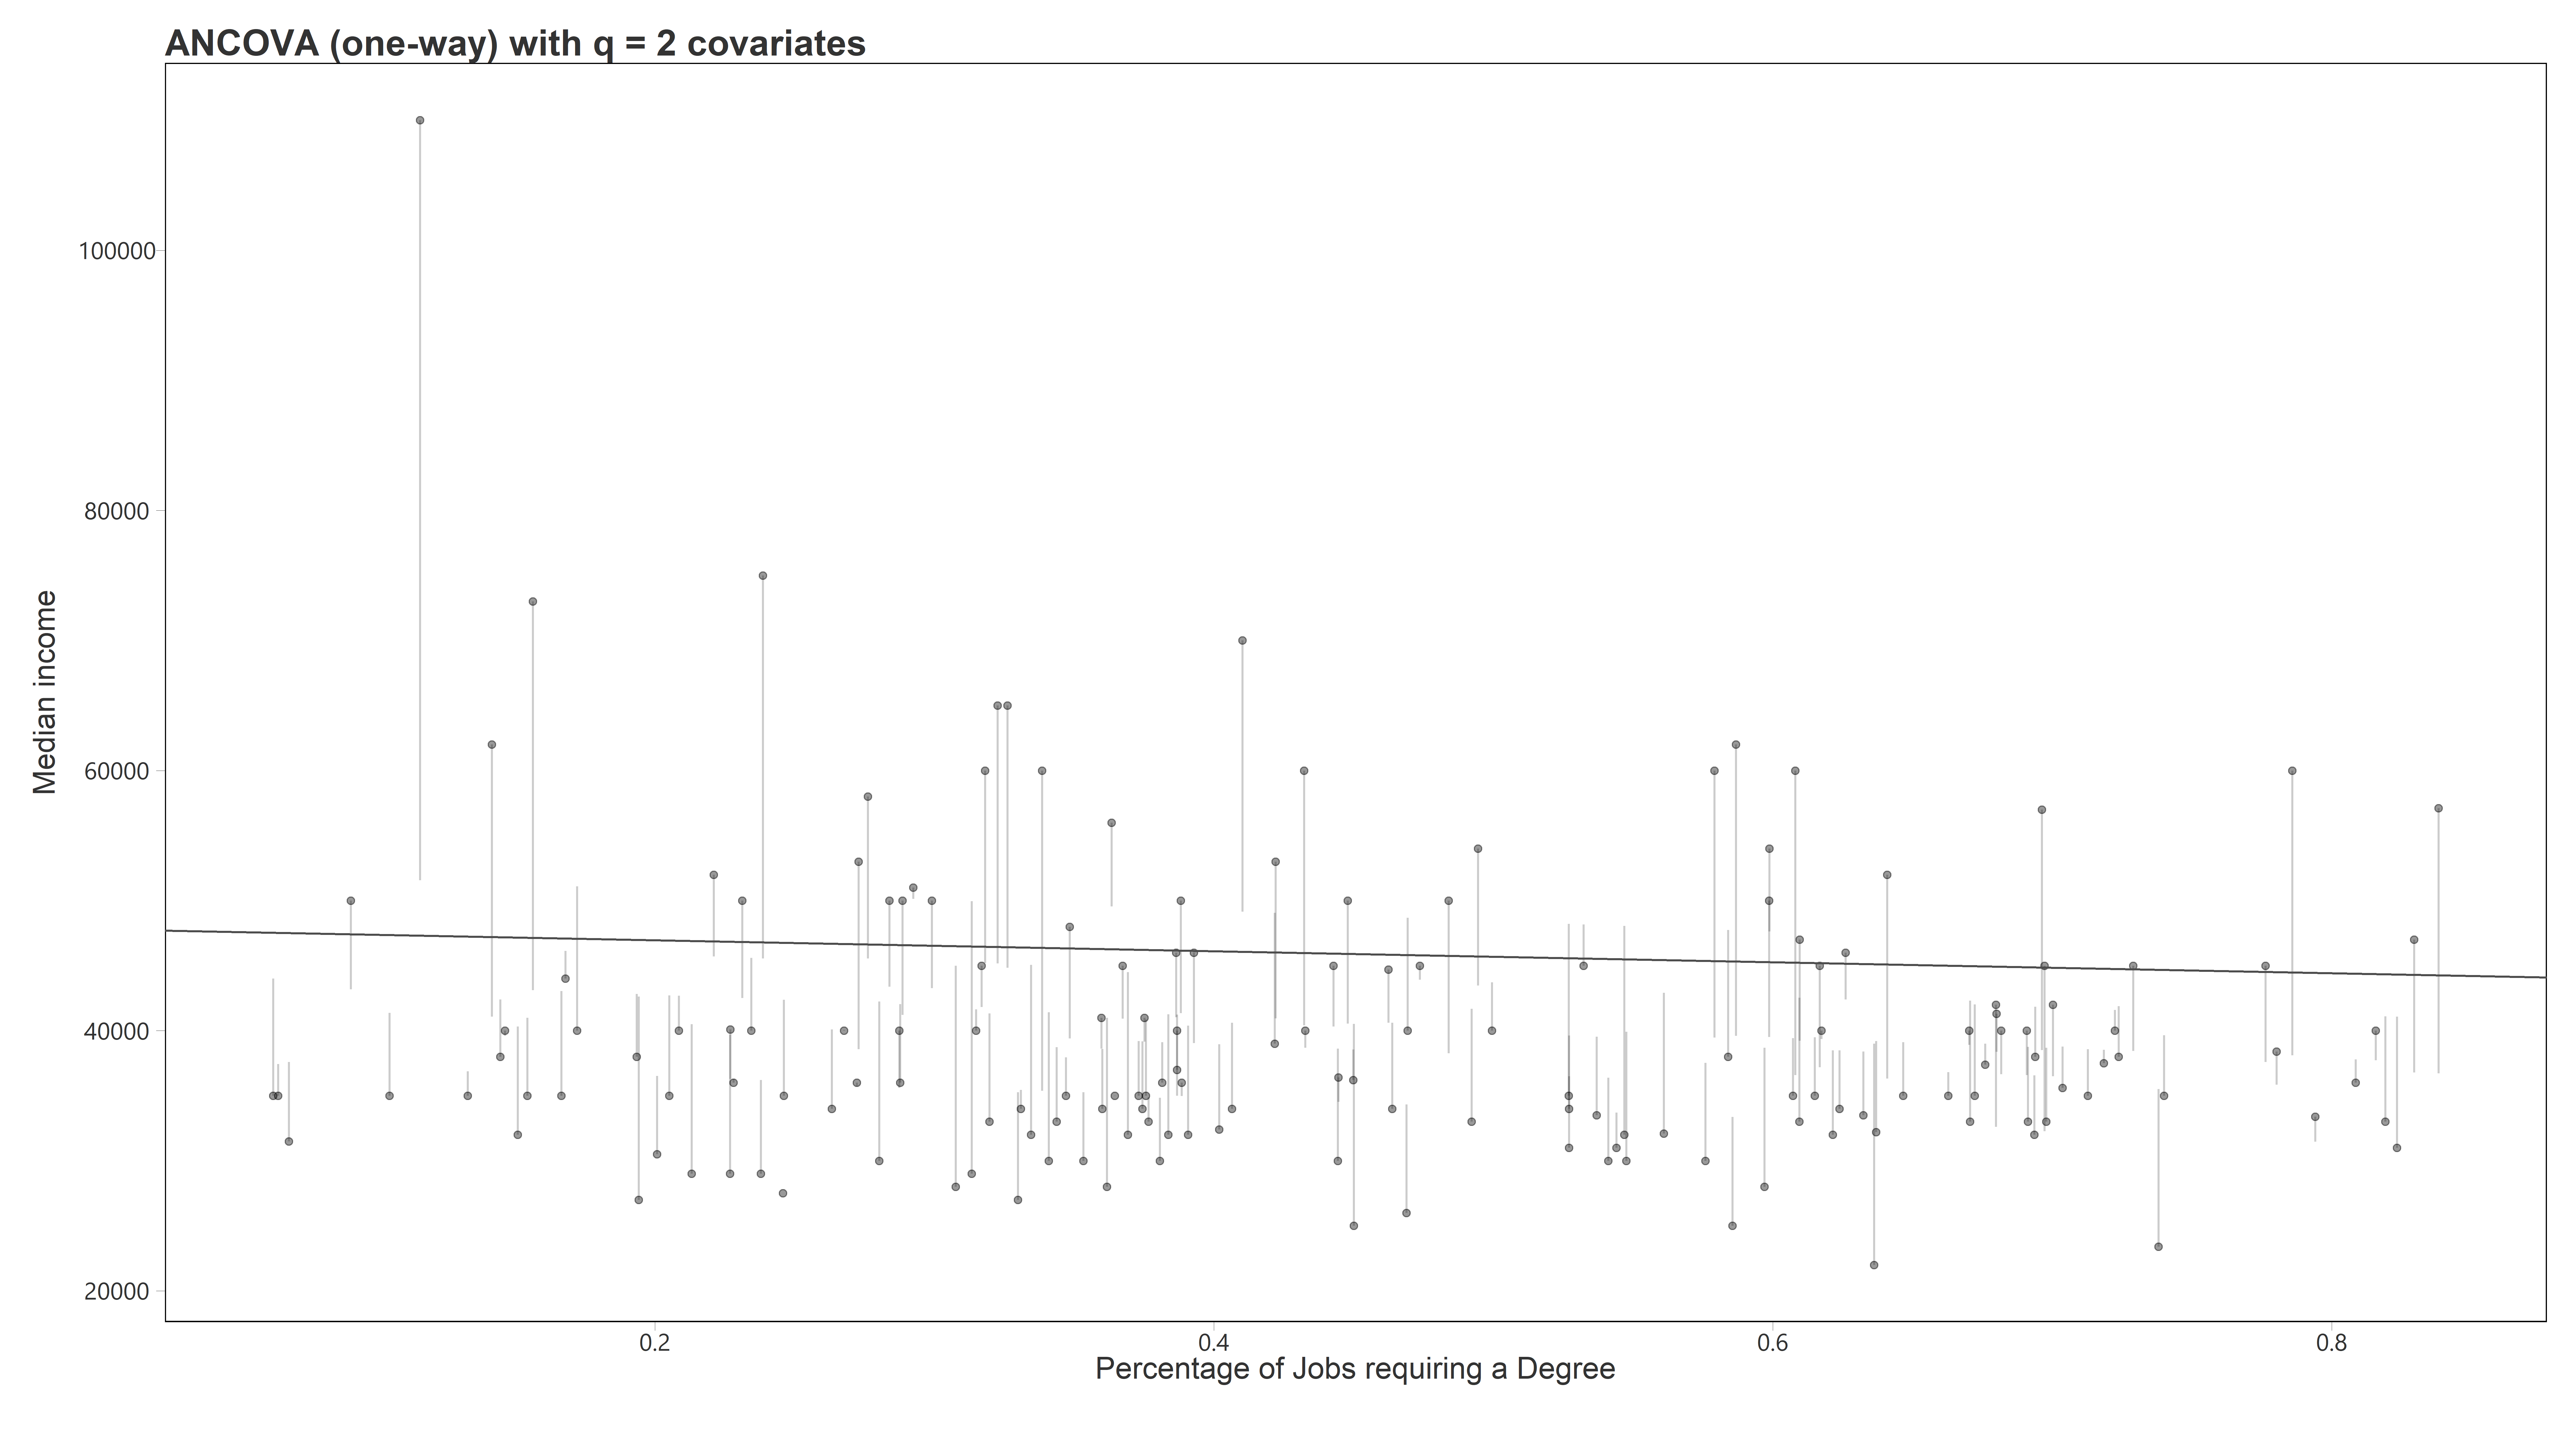
\includegraphics[scale=0.365]{plot4}
\caption{}
\end{figure}
%% -------------------------------------------------------------------------------------------|

%% [A-title] block ...
%% -------------------------------------------------------------------------------------------\
\begin{center}
\section{DISCUSSION}
\vspace{-3ex}
\end{center}
%% -------------------------------------------------------------------------------------------|

%% [B-paragraph] block ...
%% -------------------------------------------------------------------------------------------\
\noindent
\textsc{case i} revealed a weak linear relation between the regressors and
the response variable. However, \textsc{case i} resutls only
state that no \emph{linear} relation exists, but does not state that
no \emph{other} relation exists. Such a relation would require more advanced
mathematical modeling techiniques to discover what this true relation would be.
In addition, the variance inflation factors for \textbf{perc college jobs}
and \textbf{perc non college jobs} were moderatly high. This indicated that at
least one of the two features were redundant and should be removed.
\smallskip

After making adjustments to the model, the same procedure in \textsc{case i}
was conducted a second time in \textsc{case ii}. However, model validation was
skipped, given it served its purpose in \textsc{case i}. These results from the
hypothesis test reached a similar conclusion: there is no sign of linearity in
the model.
%% -------------------------------------------------------------------------------------------|
\end{document}